\chapter{Concurrent Multiscale Simulations of Nonlinear Random Materials Using Probabilistic Learning}
\label{chap:fe2}

 In this work, we explore an alternative path to address this problem and seek to construct a statistical surrogate model where the forward map of interest (specifically, the non-local constitutive model) is approximated using statistical conditioning. Instead of calibrating a regression model between the input (e.g., the deformation gradient) and the output (say, a stress measure), we aim to directly generate samples from the input-output joint probability measure, and to estimate quantities of interest through conditional means. This viewpoint requires the use of a generative model capable of accurately capturing measure concentration and the (unknown) geometry of the support of the measure in the small data limit --- a task that remains particularly challenging for strongly non-Gaussian distributions in high dimensions. We note that the construction of generative models is a vibrant topic across many scientific communities, and providing an extensive review on existing techniques is beyond the scope of this paper. In the present study, we employ probabilistic learning on manifolds (PLoM) \cite{Soize2016,Soize2020c,Soize2022a} to perform this task. The choice of this technique is motivated by (\textit{i}) its capability to sample the probability measure defined by the training dataset and in particular, to respect measure concentration and support information (as demonstrated in \cite{Farhat2019,Ghanem2019, Arnst2021,Capiez2022,Ghanem2022, Safta2022, Sinha2023, Zhong2023, Ezvan2023, Almeida2023,Govindjee2023,Soize2024}), (\textit{ii}) relative ease of implementation, and (\textit{iii}) its reliance on low-dimensional, interpretable parameterization. Our main contributions are as follows. First, we formulate the approximation of the non-local homogenized response in nonlinear elasticity as a learning problem. Second, we perform extensive numerical studies and address the validation of the framework under two scenarios relevant to inverse problem solving and forward propagation. In the former case, the approach can be used, for instance, to calibrate hyperparameters in the material model at fine scale, integrating data at the coarse scale. The latter case represents the classical surrogate setting with aleatoric uncertainties induced by subscale randomness (without separation of scales). Notice that while the proposed developments are derived in the context of nonlinear elasticity, they remain applicable to other classes of constitutive models --- at the expense of adapting the mechanistic parameterization.

This section is organized as follows. The multiscale mechanistic framework is first introduced in Section \ref{sec:mechanics}. The deterministic scale-coupling problems (and their stochastic counterparts) are presented, together with the stochastic model enabling the representation of material randomness at mesoscale. Section \ref{sec:PLoM} provides a comprehensive overview on the probabilistic learning framework, including both theoretical and algorithmic aspects. In Section \ref{sec:application}, the proposed framework is applied in the context of finite elasticity. The two aforementioned scenarios are specifically introduced to assess the robustness of the method (in probability law).

\section{Description of the Mechanistic Framework}\label{sec:mechanics}
\subsection{Definition of the Structural Problem}\label{subsec:def-struc-pb}

Let $\Omega_\text{str}$ be an open bounded domain in $\mathbb{R}^d$ (here, $d = 2$ without loss of methodological generality) representing the reference configuration for the structure of interest, and denote by $\partial \Omega_\text{str}$ the boundary of $\Omega_\text{str}$. For any material point $\bfx \in \Omega_\text{str}$, the spatial point $\bfx^\varphi$ in the deformed configuration $\Omega_{\text{str}}^\varphi$ is given by $\bfx^\varphi = \varphi (\bfx)$, where $\varphi$ is the deformation map. To make the presentation concrete, we assume that the material (at fine scale) is hyperelastic, compressible and isotropic. In addition, we consider a Saint Venant–Kirchhoff model, with a strain energy density function given by
\begin{align}
    \psi([E]) = \frac{\lambda}{2} [\textnormal{tr}([E])]^2 + \mu \, \textnormal{tr}([E]^2)\,,\label{eq: strain energy density}
\end{align}
where $\lambda$ and $\mu$ are the Lamé parameters. Note that the proposed approach can accommodate other types of constitutive behaviors, and that the above choice pertaining to the strain energy density function is not expected to impact the methodological results presented in this research. 

For any $\bfx \in \Omega_\text{str}$, the deformation gradient $[F]$ is a second-order tensor defined as $[F] = [\boldsymbol{\nabla}_{\bfx} \bfx^\varphi]$. The right Cauchy-Green deformation tensor is defined as $[C] = [F]^T [F]$, and the Green-Lagrange strain tensor defined as $[E] = \frac{1}{2}([C] - [I])$. In a general setting, the strong form (resulting from the balance of linear momentum) of the boundary value problem (BVP) in the reference configuration is stated as \cite{ciarlet}
\begin{align}
    \boldsymbol{\nabla}_{\bfx} [P(\bfx)] + \bfb(\bfx)  = \mathbf{0}\,,& \quad \forall\,\bfx \in \Omega_\text{str}\,, \label{eq: stress divergence structural}\\
    \bfu(\bfx) = \overline{\bfu}(\bfx)\,,& \quad \forall\, \bfx \in \partial \Omega_\text{str}^D\,,\\
    [P(\bfx)] \cdot \bfn(\bfx) = \overline{\bft}(\bfx)\,,& \quad \forall\, \bfx \in \partial \Omega_\text{str}^N\,,
\end{align}
where $\boldsymbol{\nabla}_{\bfx}$ denotes the divergence operator in the reference configuration, $[P]$ is the first Piola-Kirchhoff stress tensor defined as
\begin{equation}
    [P] = \frac{\partial \psi([F])}{\partial [F]}\,,
\end{equation}
the vector $\bfb$ is the body force, $\bfn$ is unit vector normal to the boundary in the reference configuration, $\overline{\bfu}$ and $\overline{\bft}$ are given smooth vector fields on the Dirichlet and Neumann boundaries, denoted by $\partial \Omega_\text{str}^D$ and $\partial \Omega_\text{str}^N$ respectively. The solution to the above problem is classically sought (in an appropriate function space) as a stationary point of the following energy functional \cite{ciarlet,wriggers2008nonlinear,bonet_wood_2008}:
\begin{align}
    \Pi(\varphi) &= \int_B \psi([F]) \, dV - \int_{B} \bfb \cdot \varphi\,dV - \int_{\partial B_N} \overline{\bft} \cdot \varphi\,dA\,.
\end{align}
In this work, we apply a Dirichlet boundary condition $\overline{\bfu}$ on $\partial \Omega_\text{str}$ (i.e., no traction is applied, and the body force is neglected).

\subsection{Definition of the Macroscopic Problem in the Context of Concurrent Multiscale Approaches}\label{subsec:def-mac-pb}

Let $\Omega_\text{mac} \subset \Omega_\text{str}$ denote the reference configuration for the subdomain where the surrogate must be constructed, and denote by $\partial \Omega_\text{mac}$ its boundary (see Fig.~\ref{fig:scales}).
\begin{figure}[!htb]
    \begin{center}
        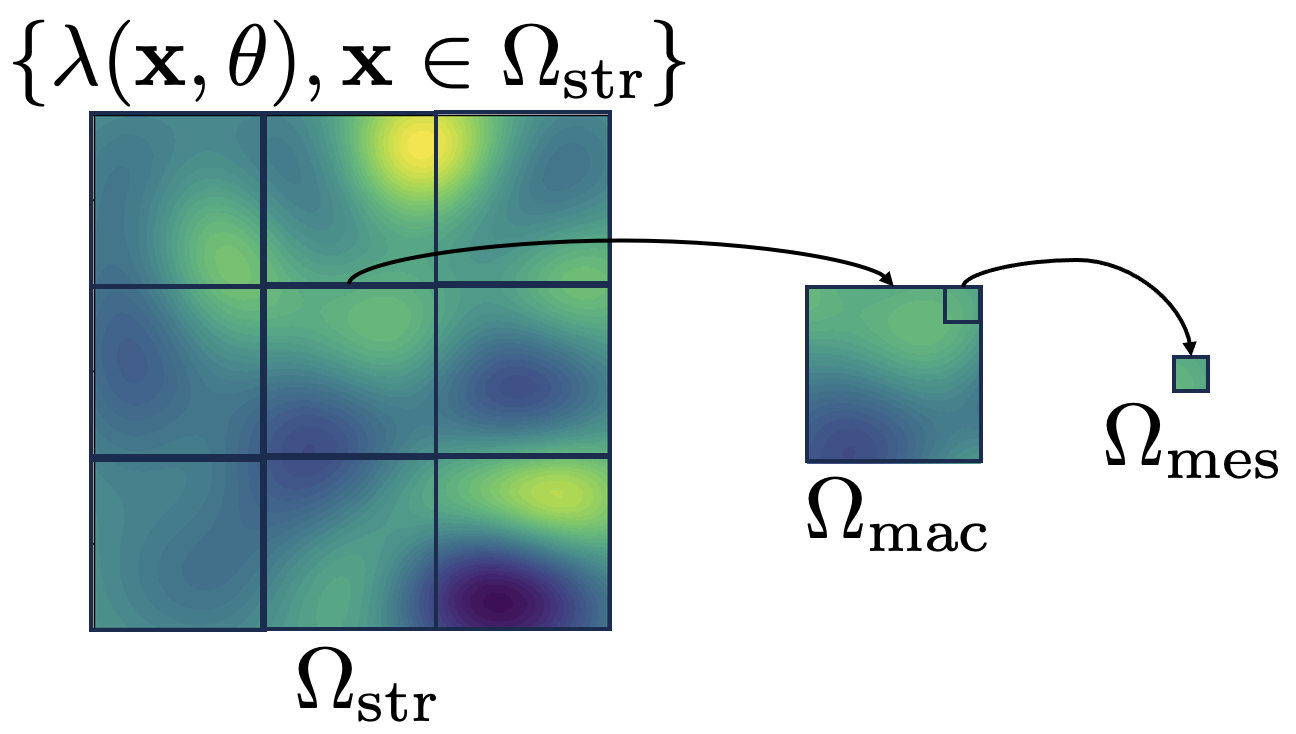
\includegraphics[width = 0.5\textwidth]{Pictures/Fig-Scales.png}
    \end{center}
    \caption[Definition of scales in the concurrent multiscale simulations.]{Definition of scales in the concurrent multiscale simulations. Fluctuations in the first Lam\'e parameter $\lambda$ are introduced at fine scale.}
    \label{fig:scales}
\end{figure}
Let $\overline{\bfu}_{\text{mac}}$ be the restriction of the solution to the structural problem (defined in the previous section) to the boundary $\partial \Omega_\text{mac}$. The strong form of the boundary value problem in the reference configuration of $\Omega_\text{mac}$ is stated as
\begin{align}
    \boldsymbol{\nabla}_{\bfx} [P_\text{mac}(\bfx)] = {\mathbf{0}}\,,& \quad \forall\,\bfx \in \Omega_\text{mac}\,,\\
    \bfu(\bfx) = \overline{\bfu}_{\text{mac}}(\bfx)\,,& \quad \forall\, \bfx \in \partial \Omega_\text{mac}\,,
\end{align}
where $[P_\text{mac}]$ is the first Piola-Kirchhoff stress tensor at macroscale. % and can be thought of as the image of the Dirichlet boundary conditions specified by $\overline{\bfu}$ through the localization operator $\curL_\text{loc}$ implicitly defined by Eq.~\eqref{eq: stress divergence structural}, $\curL_\text{loc}:\overline{\bfu} \mapsto \overline{\bfu}_{\text{mac}}$ (written in the almost sure sense).

In order to define the multiscale setting, we consider a statistical volume element $\Omega_\text{mes}(\bfx)$ located at point $\bfx \in \Omega_\text{mac}$, and denote by $\partial \Omega_\text{mes}$ the boundary of $\Omega_\text{mes}$ (as shown in Fig.~\ref{fig:scales}). Given a finite element discretization of $\Omega_\text{str}$ and at a given iteration in the nonlinear (Newton-Raphson) solver, the concurrent method proceeds by estimating the deformation gradient $[F_\text{mac}(\bfx^{q})]$ at any quadrature point $\bfx^{q}$ in $\Omega_\text{mac}$, and by evaluating the apparent first Piola-Kirchhoff stress tensor defined as
\begin{equation}
    [P_\text{mac}(\bfx^{q})] = \frac{\partial \overline{\psi}_\text{mac}([F_\text{mac}(\bfx^{q})]; \Omega_\text{mes}(\bfx^{q}))}{\partial [F_\text{mac}(\bfx^{q})]}\,,
\end{equation}
where $\overline{\psi}_\text{mac}(\cdot; \Omega_\text{mes}(\bfx^{q}))$ is the apparent strain energy density function associated with the mesoscopic domain $\Omega_\text{mes}(\bfx^{q})$, using localization (through $[F_\text{mac}(\bfx^{q})]$) and homogenization (via $\overline{\psi}_\text{mac}(\cdot; \Omega_\text{mes}(\bfx^{q}))$). Note that as previously pointed out, scale separation is not enforced and thus, all quantities obtained by upscaling are termed \textit{apparent}, following the convention introduced by Huet \cite{HUET1990813} (see also \cite{book-ostoja}). In order to compute $[P_\text{mac}]$ at each quadrature point $\bfx^{q} \in \Omega_\text{mac}$, we use the FE$^2$ method \cite{feyel2000fe2, feyel2003multilevel} and solve the boundary value problem defined as
\begin{align}
    \boldsymbol{\nabla}_{\bfx} [P_\text{mes}(\bfx)] = {\mathbf{0}}\,,& \quad \forall\,\bfx \in \Omega_\text{mes}(\bfx^{q})\,,\\
    \bfu(\bfx) = ([F_\text{mac}(\bfx^{q})] - [I]) \bfx \,,& \quad \forall\, \bfx \in \partial \Omega_\text{mes}(\bfx^{q})\,,
\end{align}
in the reference configuration of $\Omega_\text{mes}(\bfx^{q})$, where $[F_\text{mac}(\bfx^{q})]$ is the deformation gradient inherited from the macroscale boundary value problem at $\bfx^{q}$. The apparent first Piola-Kirchhoff stress tensor at $\bfx^{q}$ is then evaluated as \cite{hill1972constitutive}
\begin{align}
    [P_\text{mac}(\bfx^{q})] = \frac{1}{\vert\Omega_\text{mes}(\bfx^{q})\vert} \int_{\Omega_\text{mes}(\bfx^{q})} [P_\text{mes}(\bfx)]\,d\bfx\,.
\end{align}
As we will explain in the next section, the pairs of associated deformation gradients and first Piola-Kirchhoff stress tensors at all quadrature points in the macroscopic domain $\Omega_\text{mac}$ are then used to compute the pairs of associated right Cauchy-Green deformation tensors and second Piola-Kirchhoff stress tensors, which are the (objective) mechanistic variables considered in the probabilistic learning process introduced in Section \ref{sec:PLoM}. Note that while the deformation gradient and the first Piola-Kirchhoff stress tensor could also be used in the learning approach, the choice of the right Cauchy-Green deformation tensor and second Piola-Kirchhoff stress tensor as quantities of interest leads to smaller dimensions since both tensors are symmetric. It should also be pointed out that preserving mechanical variables over the entire domain (namely, $\Omega_\text{mac}$) enables the consideration of a nonlocal apparent constitutive model, as opposed to the calibration of a surrogate at one particular point in the domain (which is more relevant to local constitutive models).

\subsection{Description of Material Uncertainties}\label{subsec:material-model}
\subsubsection{Definition of the Stochastic Model}
\label{subsubsec:sto-model}
In this section, we detail the construction of the stochastic model for the strain energy density function defined by Eq.~\eqref{eq: strain energy density}. Given the scope of this work, which is focused on the learning perspective rather than stochastic modeling, the hyperelastic model is randomized by defining the first Lam\'e parameter, $\lambda$, as a random field. Models enabling the randomization of all parameters in various classes of strain energy density functions can be found in the references provided after Eq.~\eqref{eq:def-transport}, and in \cite{JE-2013,STABER2017399} for linear elasticity (for all symmetry classes). We also note that results published elsewhere reporting on the (first-order) marginal cross-correlation of elastic moduli suggest that one latent random field may be sufficient to induce multiscale-informed stochasticity in the isotropic case (depending on the material under consideration; see, e.g., \cite{Hun2019} for a reinforced composite material).

The first Lam\'e parameter random field is denoted by $\{\lambda(\bfx), \bfx \in \Omega_{\text{str}}\}$, is defined on probability space $(\Theta,\curT,\curP)$, and takes values in $\mathbb{R}_*^+$. In this paper, we define $\{\lambda(\bfx), \bfx \in \Omega_{\text{str}}\}$ as 
\begin{equation}
    \lambda(\bfx) = \curH \left(\Xi(\bfx)\right)\,, \quad \forall \bfx \in \Omega_{\text{str}}\,,
\end{equation}
where $\curH$ denotes a so-called transport map, constructed to enforce admissibility (in the almost sure sense), and $\{\Xi(\bfx), \bfx \in \mathbb{R}^d\}$ is a centered homogeneous Gaussian random field. This Gaussian field is completely defined by its correlation function $(\bfx, \bfx') \mapsto \rho(\bfx,\bfx') = E\{\Xi(\bfx)\Xi(\bfx')\}$, which is taken as
\begin{equation}
    \rho(\bfx,\bfx') = \prod_{i = 1}^d \exp\left(-\left(\frac{x_i - x_i'}{\ell_c}\right)^2 \right)\,, \quad \forall (\bfx,\bfx') \in \mathbb{R}^d \times \mathbb{R}^d\,,
\end{equation}
for the sake of illustration, with $\ell_c$ a model parameter such that $\int_0^{+\infty} \exp\left(-(\tau/\ell_c)^2\right)\,d\tau = L_c$, where $L_c$ is the spatial correlation length of the Gaussian random field (which is assumed to be independent of the direction, for simplicity). Following the methodology introduced in \cite{SOIZE200626} in the context of anisotropic linear elasticity, the transport map is constructed using information theory and the principle of maximum entropy \cite{Shannon1948,Jaynes1957a,Jaynes1957b}; see \cite{Soize-book} for an introduction to concepts and methodologies, as well as \cite{GUILLEMINOT2020385} for specific results in (linear and nonlinear) mechanics of materials. Specifically, $\curH$ is defined by imposing that
\begin{equation}\label{eq:def-transport}
    \lambda(\bfx) = \curH \left(\Xi(\bfx)\right) \sim P_{\text{ME}}\,, \quad \forall \bfx \in \Omega_{\text{str}}\,,
\end{equation}
where $P_{\text{ME}}$ is the probability measure induced by entropy maximization under constraints. General methodologies and information-theoretic results for a large class of models in nonlinear elasticity can be found in \cite{staber2015cras} and \cite{Staber2017zamm}, for the cases of isotropic incompressible and compressible materials, respectively. Extensions to spatially-dependent anisotropic hyperelastic models can be found in \cite{STABER201894,CHEN2022114897}, and applications including calibration and validation using experimental data are available in \cite{STABER2017743,staber2019stochastic,CHEN2022114897} (see also \cite{mihai-book} and the references therein for a review of applications to canonical mechanics problems). Since $\lambda$ corresponds to an elasticity parameter, results obtained in the context of stochastic linearized elasticity can also be invoked. Accounting for the positiveness constraint, as well as for the existence of second-order moments for the linearized elasticity tensor and its inverse \cite{SOIZE200626,GuilleminotSoize2017}, it can be shown that $P_{\text{ME}}$ corresponds to a Gamma distribution. Denoting by $\underline{\lambda}$ and $\delta_{\lambda}$ the mean and coefficient of variation of $\lambda$, it follows that
\begin{equation}
    \curH = F_{\curG(\delta_{\lambda}^{-2},\underline{\lambda}\delta_{\lambda}^{-2})}^{-1} \circ F_{\curN(0,1)}\,,
\end{equation}
where $F_{\curG}^{-1}$ is the inverse cumulative distribution function of the Gamma distribution with shape and scale parameters given by $\delta_{\lambda}^{-2}$ and $\underline{\lambda}\delta_{\lambda}^{-2}$, respectively, and $F_{\curN(0,1)}$ is the cumulative distribution function of the standard Gaussian distribution. Notice that these hyperparameters can be made spatially-dependent to improve expressiveness in the model: this sophistication is, however, irrelevant for the objectives pursued in this paper. 

In the applications presented below, the underlying Gaussian random field $\{\Xi(\bfx), \bfx \in \mathbb{R}^d\}$ is sampled using a truncated Karhunen-Lo\`eve expansion, with an order of truncation determined such that the $L^2$ error falls below a given threshold (chosen as $1\mathrm{e}{-2}$). Samples for both the Gaussian and non-Gaussian random fields are shown in Fig.~\ref{fig:samples}, for $\underline{\lambda} = 40\,000$, $\delta_{\lambda} = 0.2$, and $L_c = 0.3$.
\begin{figure}[!htb]
    \begin{center}
        \subfloat[Sample of $\{\Xi(\bfx), \bfx \in \Omega_{\text{str}}\}$.]{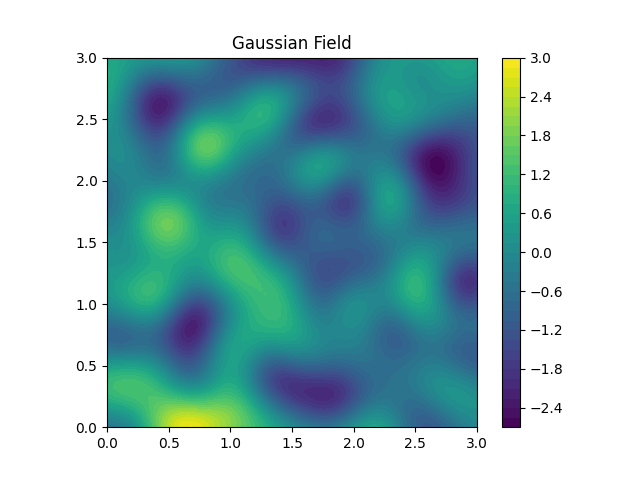
\includegraphics[width=0.44\textwidth]{Pictures/Gaussian_sample_1.png}}
    \hspace{0.05\textwidth}
    \subfloat[Sample of $\{\lambda(\bfx), \bfx \in \Omega_{\text{str}}\}$ computed from (a).]{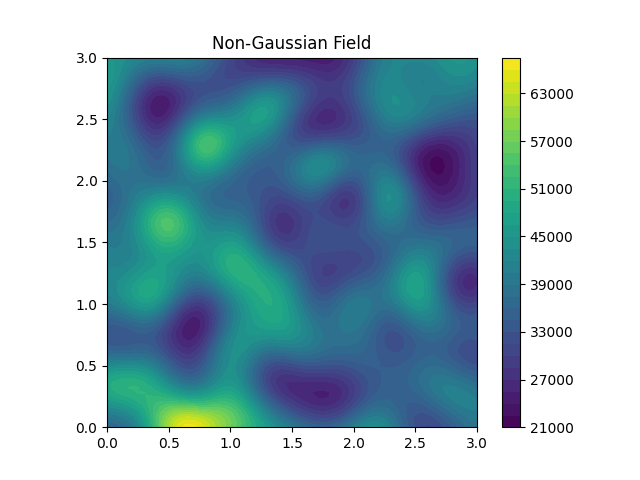
\includegraphics[width=0.44\textwidth]{Pictures/NonGaussian_sample_1.png}}
    \end{center}
    \caption[Realizations of the underlying Gaussian field and material parameter random field.]{Realizations of the underlying Gaussian field (left) and material parameter random field (right).}
    \label{fig:samples}
\end{figure}

\subsubsection{Definition of the Stochastic Boundary Value Problems}
Considering the Lam\'e parameter random field defined in Section \ref{subsubsec:sto-model} in the BVPs introduced in Sections \ref{subsec:def-struc-pb} and \ref{subsec:def-mac-pb} leads to the definition of stochastic boundary value problems (SBVPs), which are briefly described below for the sake of readability. All equalities below hold in the almost sure sense.

Following the retained modeling setup, the structural stochastic boundary value problem is given by
\begin{align}
    \boldsymbol{\nabla}_{\bfx} [\bfP(\bfx)]  = \mathbf{0}\,,& \quad \forall\,\bfx \in \Omega_\text{str}\,,\\
    \bfU(\bfx) = \overline{\bfu}(\bfx)\,,& \quad \forall\, \bfx \in \partial \Omega_\text{str}^D\,,\label{eq: structural-sto-bc}
\end{align}
where $[\bfP]$ is the stochastic Piola-Kirchhoff stress tensor (arising from the randomization of the strain energy density function via $\lambda$), $\{\bfU(\bfx),\bfx\in \Omega_\text{str}\}$ is the displacement solution random field and $\bfx \mapsto \overline{\bfu}(\bfx)$ is the known deterministic field introduced in Section \ref{subsec:def-struc-pb}. Similarly, the macroscopic SBVP on the domain of interest $\Omega_\text{mac}$ (where the statistical surrogate is built) writes
\begin{align}
    \boldsymbol{\nabla}_{\bfx} [\bfP_\text{mac}(\bfx)] = {\mathbf{0}}\,,& \quad \forall\,\bfx \in \Omega_\text{mac}\,,\\
    \bfU(\bfx) = \overline{\bfU}_{\text{mac}}(\bfx)\,,& \quad \forall\, \bfx \in \partial \Omega_\text{mac}\,,
\end{align}
where $\{\overline{\bfU}_{\text{mac}}(\bfx), \bfx \in \partial \Omega_\text{mac}\}$ is now a random field with values in $\mathbb{R}^d$, due to the fact that the background medium is stochastic. Finally, the SBVP considered in the concurrent approach (for any subdomain $\Omega_\text{mes}(\bfx^{q})$ centered at quadrature point $\bfx^{q}$ in $\Omega_\text{mac}$) is
\begin{align}
    \boldsymbol{\nabla}_{\bfx} [\bfP_\text{mes}(\bfx)] = {\mathbf{0}}\,,& \quad \forall\,\bfx \in \Omega_\text{mes}(\bfx^{q})\,,\\
    \bfU(\bfx) = ([\bfF_\text{mac}(\bfx^{q})] - [I]) \bfx \,,& \quad \forall\, \bfx \in \partial \Omega_\text{mes}(\bfx^{q})\,,
\end{align}
where $[\bfF_\text{mac}(\bfx^{q})]$ is the stochastic deformation gradient at $\bfx^{q}$, defined through localization.

In this work, we consider the strong stochastic solutions to the weak formulations (using the Galerkin method and a finite element discretization) of the above SBVPs. The Monte Carlo approach is chosen as the stochastic solver. The pairs of right Cauchy-Green deformation tensors and second Piola-Kirchhoff stress tensors (denoted by $\{[C_\text{mac}(\bfx^{q})],[S_\text{mac}(\bfx^{q})]\}_{q = 1}^{Q_\text{mac}}$) are collected at all quadrature points, for all samples of the Lam\'e parameter random field, to constitute the dataset for the probabilistic learning procedure introduced in Section \ref{sec:PLoM}.

\subsection[Implementation Verification for the FE2 Method (With Deterministic Background Media)]{Implementation Verification for the FE\,$^2$ Method (With Deterministic Background Media)}
For the sake of illustration, we consider the structural domain $\Omega_{\text{str}} = [0, 3]^2$, and define the macroscopic domain of interest as $\Omega_{\text{mac}} = [1, 2]^2$. The mesoscopic domain $\Omega_{\text{mes}}(\bfx^{q})$ at quadrature point $\bfx^{q}$ is defined by a characteristic length $L_{\Omega_{\text{mes}}} = 0.025$. Spatial discretization is realized using Q4 elements at all mesh resolutions. The number of elements per direction is 15 in $\Omega_\text{str}$, 5 in $\Omega_\text{mac}$, and 5 in $\Omega_{\text{mes}}$. The Dirichlet boundary conditions applied on the boundary of $\Omega_{\text{str}}$ are given by
\begin{align}
    \overline{\bfu}(\bfx) = \mathbf{0}\,, \quad x_1 = 0\,, \quad \forall x_2 \in [0,3]\,,\\
    \overline{\bfu}(\bfx) = \begin{bmatrix}
        0.1 \\ 0 \end{bmatrix}, \quad x_1 = 3\,, \quad \forall x_2 \in [0,3]\,.
\end{align}
As described in the previous section, the solution vector $\bfu$ in $\Omega_\text{str}$ along the boundary $\partial \Omega_\text{mac}$ of $\Omega_\text{mac}$ is applied as the Dirichlet boundary condition for the multi-scale problem. 

Implementation was performed within the MOOSE finite element framework \cite{permann2020moose}. A convergence study on the solution on $\Omega_\text{str}$ was first conducted. The solution obtained with a very fine mesh containing 960 elements per direction was used, with material parameters given by $\lambda = 40\,000$ [kg/cm$^2$] and $\mu = 10\,000$ [kg/cm$^2$] (these values, taken from \cite{picinbono2003non}, correspond to a soft biological tissue, modeled as a Saint Venant–Kirchhoff material). Regarding numerical solving, a standard Newton-Raphson solver was used with a maximum number of nonlinear iterations set to 25, with a relative tolerance taken as $1\mathrm{e}{-10}$, and an absolute tolerance given by $1\mathrm{e}{-12}$. The convergence order is measured by the $L^2$-norm of the difference between the approximation $u^h$ and the reference solution $u^{\text{ref}}$ within the domain $[1, 2]^2$. Standard $h$-convergence is observed, as illustrated in Fig.~\ref{fig:convergence}.
\begin{figure}[!htb]
    \begin{center}
        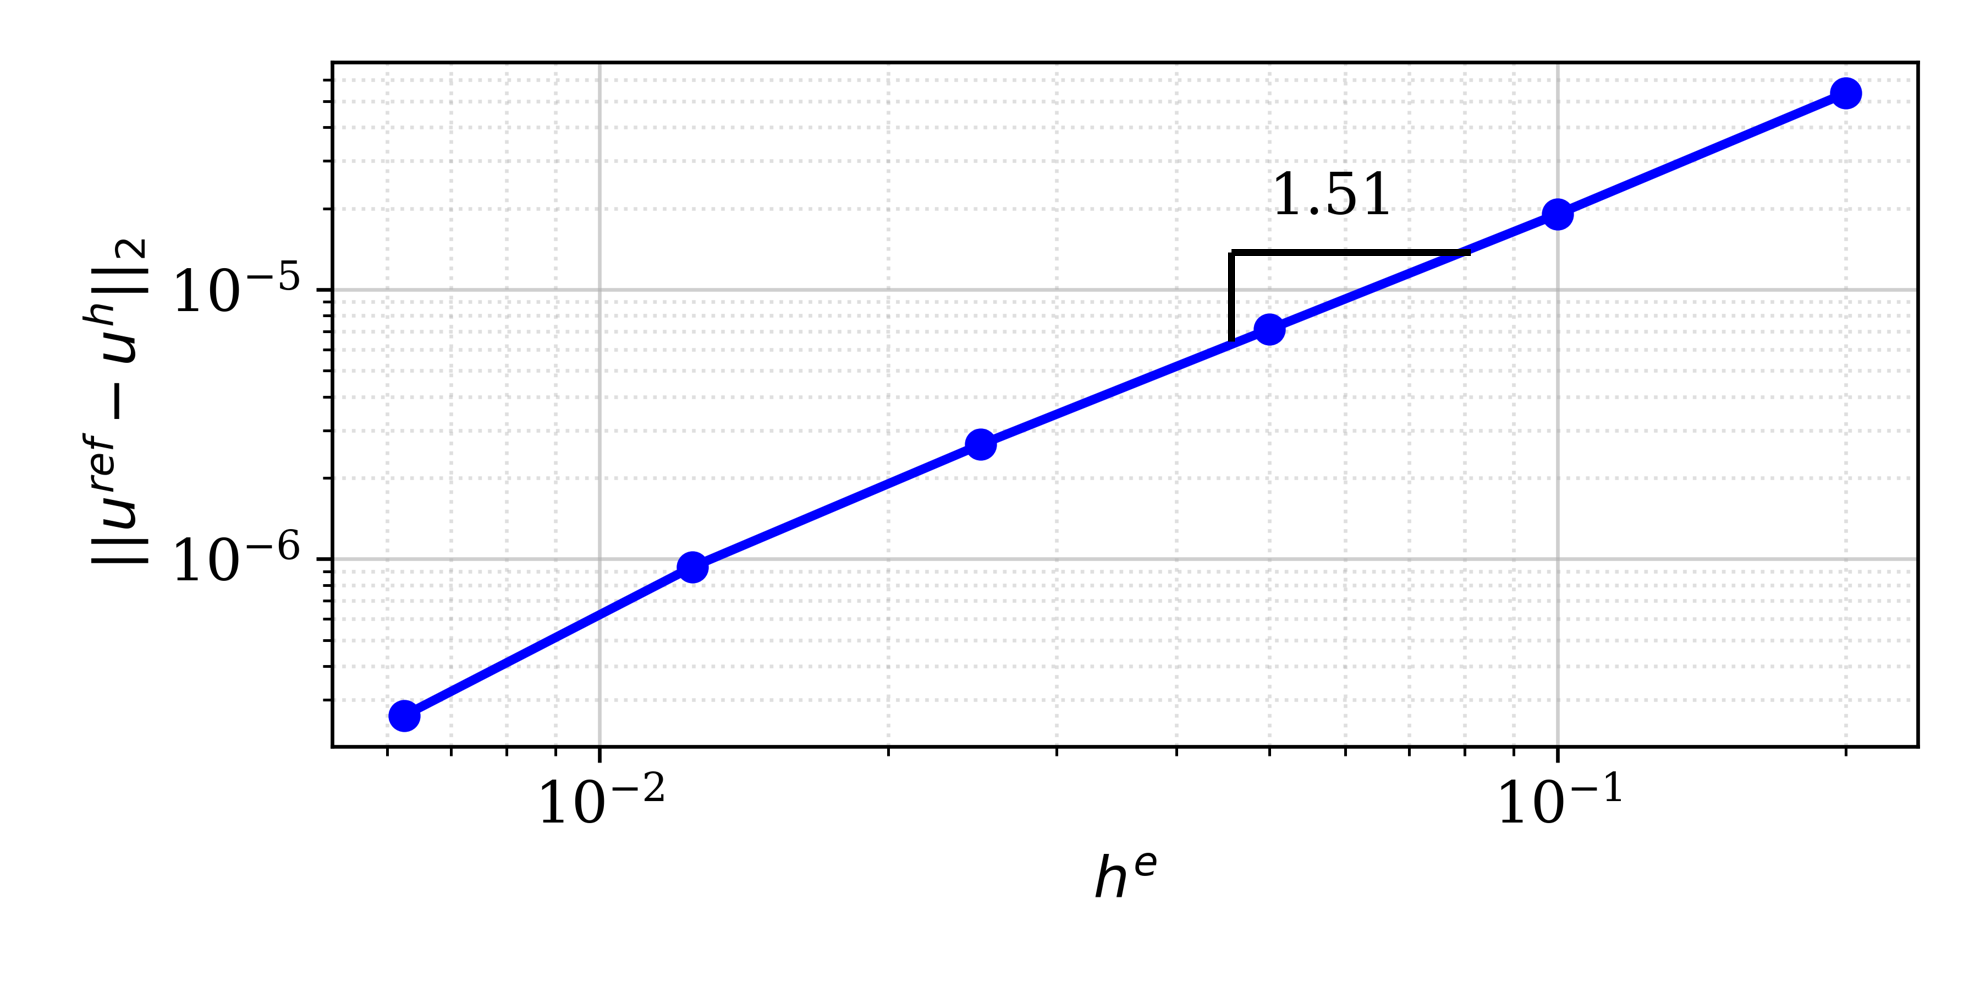
\includegraphics[width = 0.5\textwidth]{Pictures/convergence.png}
    \end{center}
    \caption[Convergence of the $L^2$ error ($h$-refinement) for the reference solution.]{Convergence of the $L^2$ error ($h$-refinement) for the reference solution.}
    \label{fig:convergence}
\end{figure}

Next, the implementation of the FE$^2$ method was verified by comparing the normalized $L^2$-norm error between the solution vector (at all nodes) on $\Omega_\text{str}$ without multiscale coupling, and the solution vector (at all nodes) obtained by using the FE$^2$ method in the subdomain $\Omega_\text{mac} = [1, 2]^2$. Fig.~\ref{fig:validation} shows the first sample of the material random field $\lambda$ (for $\underline{\lambda} = 40\,000$, $\delta_{\lambda} = 0.2$, and $L_c = 0.3$), as well as solutions to the structural and macroscale problems. 
\begin{figure}[!htb]
    \begin{center}
        \begin{subfigure}[b]{0.32\textwidth}
            \begin{center}
                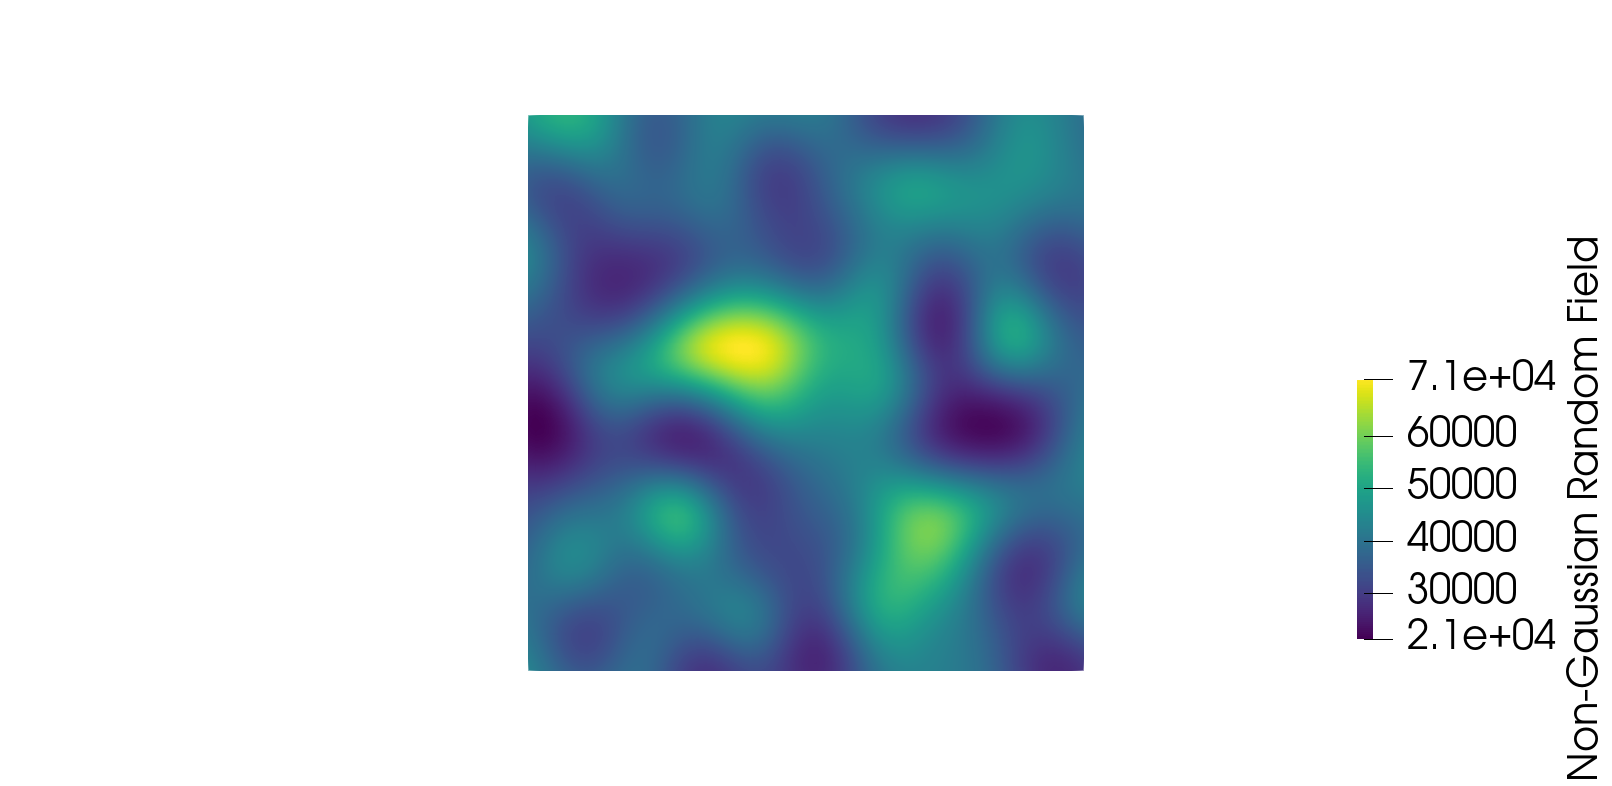
\includegraphics[trim = {12cm 0cm 0cm 0cm}, clip, width=\textwidth]{Pictures/lambda_11.png}
            \end{center}
            \caption{$\{\lambda(\bfx, \theta), \bfx \in \Omega_{\text{str}}\}$}
        \end{subfigure}
        \begin{subfigure}[b]{0.32\textwidth}
            \begin{center}
                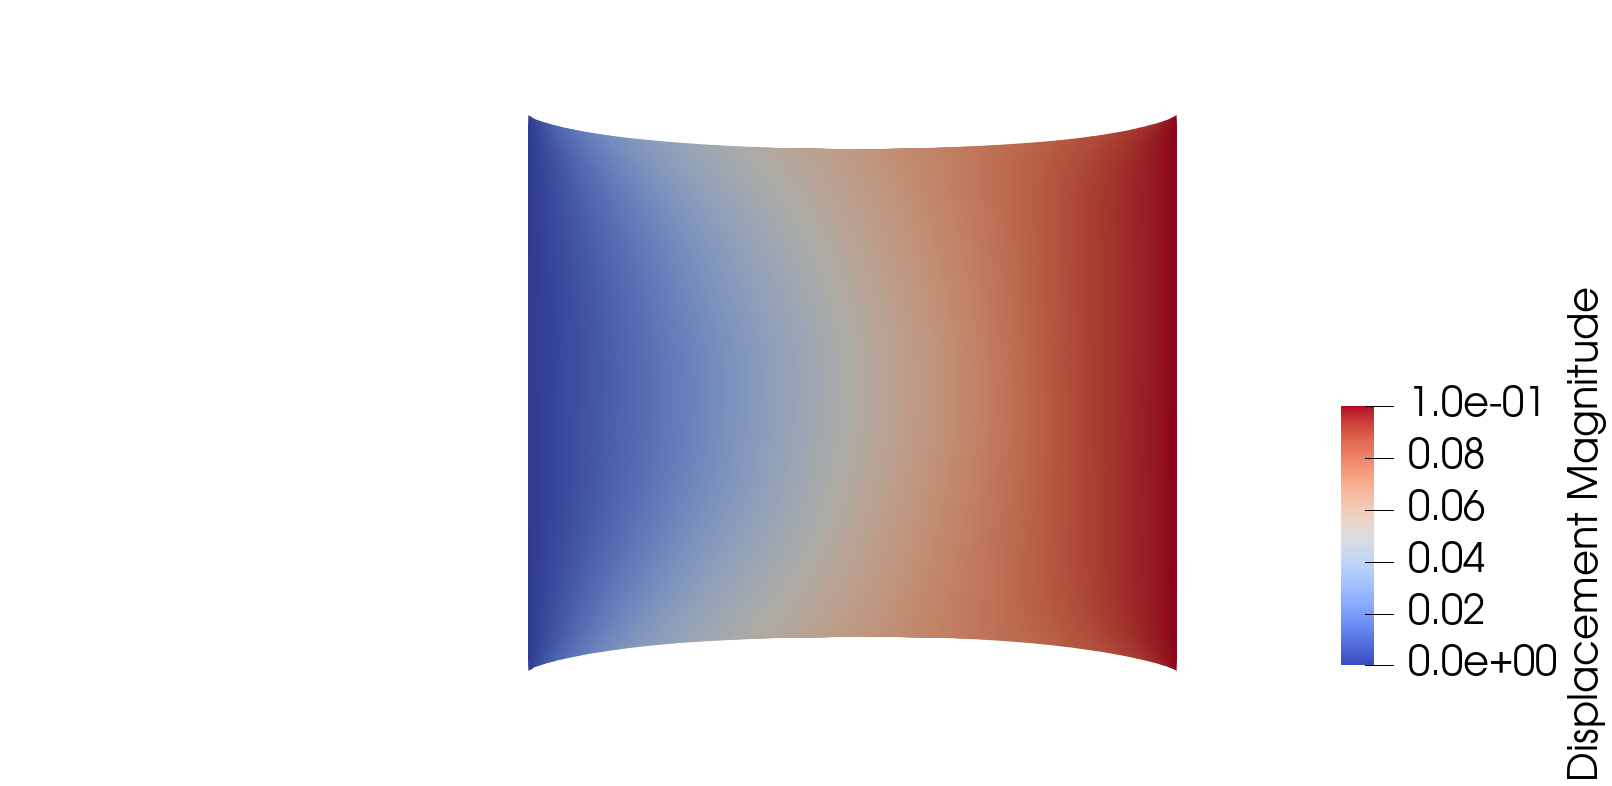
\includegraphics[trim = {12cm 0cm 0cm 0cm}, clip, width=\textwidth]{Pictures/omega_str_11.png}
            \end{center}
            \caption{$\bfx \mapsto \lVert \bfu_\text{str}(\bfx)\rVert$}
        \end{subfigure}
        \begin{subfigure}[b]{0.32\textwidth}
            \begin{center}
                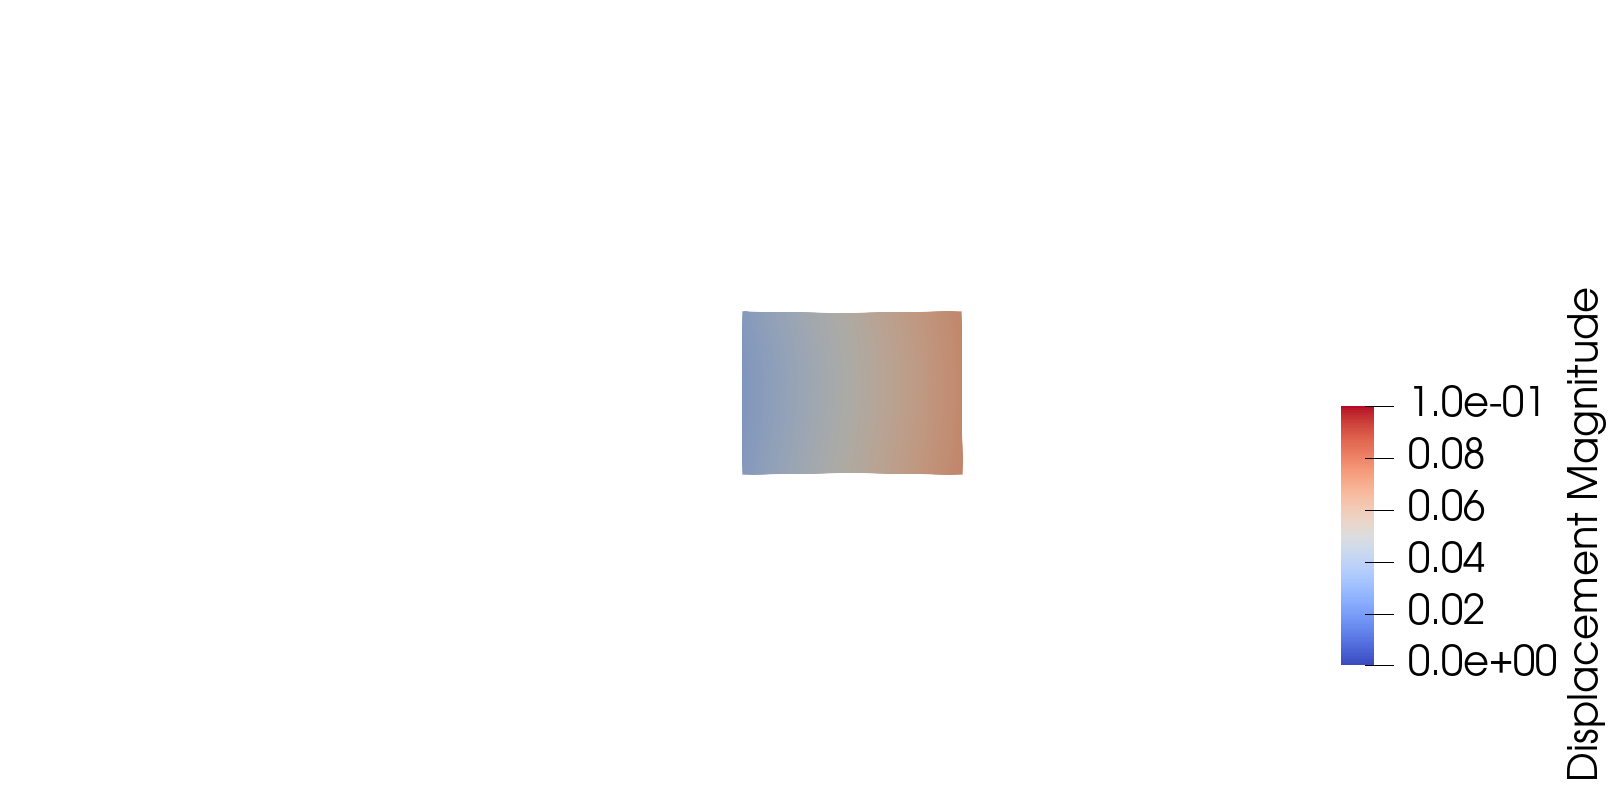
\includegraphics[trim = {12cm 0cm 0cm 0cm}, clip, width=\textwidth]{Pictures/omega_mac_11.png}
            \end{center}
            \caption{$\bfx \mapsto \lVert \bfu_\text{FE$^2$}(\bfx)\rVert$}
        \end{subfigure}
    \end{center}
    \caption[Sample of the material parameter and associated displacement magnitudes for the solutions on macroscopic and mesoscopic scale.]{Sample of the material parameter $\lambda$ (left) and associated displacement magnitudes for the solutions on $\Omega_\text{str}$ (middle) and $\Omega_\text{mac}$ (right).}
    \label{fig:validation}
\end{figure}
In order to perform a statistical analysis on the error, 500 independent samples of $\lambda$ were generated. The mean of the normalized $L^2$ error is $4.69\mathrm{e}{-4}$, and the coefficient of variation is 0.22. The probability density function of the normalized $L^2$ norm error is shown in Fig.~\ref{fig:normalized_l2_norm_distribution}.
\begin{figure}[!htb]
    \begin{center}
        \includegraphics[width=0.5\textwidth]{Pictures/l2_norm_scenario_2.pdf}
    \end{center}
    \caption[Probability density function of the normalized $L^2$-norm error.]{Probability density function of the normalized $L^2$-norm error (estimated with 500 samples).}
    \label{fig:normalized_l2_norm_distribution}
\end{figure}
These results indicate proper implementation of the concurrent multiscale method, which is used to build the dataset for the probabilistic learning technique (introduced in the next section).

\section{Overview of the Probabilistic Learning on Manifolds (PLoM) Algorithm and its Parameterization}
\label{sec:PLoM}
%----------------------------------------------------------------------------------------------------------------------------------------------
In this section, we provide a succinct overview of the PLoM algorithm, aiming to assist readers in analyzing and comprehending the underlying parameterization (which is necessary to properly interpret the presented results).

The PLoM approach~\cite{Soize2016,Soize2020c,Soize2022a} starts with the consideration of a training dataset $\curD_d$, comprising a relatively small number $n_d$ of points generated from an underlying stochastic manifold associated with a $\RR^{n}$-valued random variable $\bfX = (\bfQ,\bfW)$, defined on a probability space $(\Theta,\curT,\curP)$. Here, $\bfQ$ represents the quantity of interest and is a $\RR^{n_q}$-valued random variable, while $\bfW$ denotes the control parameter and is a $\RR^{n_w}$-valued random variable. The total dimension is $n=n_q+n_w$.
%
Another $\RR^{n_u}$-valued random variable $\UU$, defined on $(\Theta,\curT,\curP)$, is also considered as an uncontrolled parameter. The random variable $\bfQ$ is assumed to be expressed as $\bfQ = \bff(\UU,\bfW)$, where the measurable mapping $\bff$ is not explicitly known. The joint probability distribution $P_{\bfW,\UU}(d\bfw,d\uu)$ of  $\bfW$ and $\UU$ is assumed to be given. The non-Gaussian probability measure $P_{\bfX}(\bfx) = P_{\bfQ,\bfW}(d\bfq,d\bfw)$ of $\bfX =(\bfQ,\bfW)$ is concentrated in a region of $\RR^{n}$, for which the only available information is the cloud of points in the training dataset $\curD_d$. The PLoM method enables the generation of  the learned dataset $\curD_{\ar}$ for $\bfX$, consisting of $n_{\pMC} \gg n_d$ points (learned realizations) generated by the non-Gaussian probability measure estimated using the training dataset.
%
The preservation of the probability measure concentration is guaranteed by the utilization of a diffusion-maps basis, which enriches the available information from the training dataset. Utilizing the learned dataset $\curD_\ar$, PLoM enables the computation of conditional statistics, such as $\bfw\mapsto P_{\bfO\vert \bfW}(d\bfo\vert\bfW=\bfw)$, on $\curC_w$. Here, $\bfO = \bfxi(\bfQ)$, where $\bfxi$ is a measurable mapping from $\RR^{n_q}$ into $\RR^{n_o}$, allowing for the construction of statistical surrogate models (metamodels) within a probabilistic framework. The formulas for the computation of conditional mathematical expectations, conditional probability density functions, and conditional cumulative distribution functions, given any $\bfw_0$ in $\curC_w$, are given in \ref{app:fe2}.

The training dataset $\curD_d$ comprises $n_d$ independent realizations $\bfx_d^j= (\bfq_d^j,\bfw_d^j)$ in $\RR^{n} = \RR^{n_q}\times \RR^{n_w}$ for $j\in\{1,\ldots , n_d\}$ of random variable $\bfX=(\bfQ,\bfW)$, in which $\bfq_d^j= \bff(\uu_d^j,\bfw_d^j)$. The PLoM method allows for generating the learned dataset $\curD_\ar$, consisting of $n_\ar\gg n_d$  learned realizations $\{\bfx_\ar^{\ell},\ell = 1, \ldots ,n_\ar\}$ of random vector $\bfX$.
Once the learned dataset is constructed, the learned realizations for $\bfQ$ and $\bfW$ can be extracted as $(\bfq_\ar^\ell,\bfw_\ar^\ell) = \bfx_\ar^\ell$ for $\ell = 1, \ldots ,n_\ar$.

\subsection{Construction of a Reduced Representation}
\label{sec:PLoM.1}
%
The $n_d$ independent realizations $\{\bfx_d^j , j=1,\ldots , n_d\}$ are represented by the matrix $[x_d]= [\bfx_d^1 \ldots \bfx_d^{n_d}]$ in $\MM_{n,n_d}$. Let $[\bfX]= [\bfX^1,\ldots ,\bfX^{n_d}]$ be the random matrix with values in $\MM_{n,n_d}$, where its columns are $n_d$ independent copies of random vector $\bfX$. Utilizing Principal Component Analysis (PCA) of $\bfX$, random matrix $[\bfX]$ is written as,
%
\begin{equation}\label{eqPLoM1}
[\bfX] = [\underline x] + [\varphi]\, [\mu]^{1/2}\, [\bfH]\, ,
\end{equation}
%
where $[\bfH] = [\bfH^1,\ldots ,$ $\bfH^{n_d}]$ is a $\MM_{\nu,n_d}$-valued random matrix ($\nu\leq n$), and $[\mu]$ is the $(\nu\times\nu)$ diagonal matrix of the $\nu$ positive eigenvalues of the empirical estimate of the covariance matrix of $\bfX$. The $(n\times\nu)$ matrix $[\varphi]$ consists of the associated eigenvectors such $[\varphi]^T\,[\varphi]= [I_{\nu}]$. The matrix $[\underline x]$ in $\MM_{n,n_d}$ has identical columns, each being equal to the empirical estimate $\underline\bfx\in\RR^{n}$ of the mean value of random vector $\bfX$. The columns of $[\bfH]$ are $n_d$ independent copies of a random vector $\bfH$ with values in $\RR^{\nu}$, satisfying the normalization conditions, $E\{\bfH\}=\bfzero_\nu$ and $E\{\bfH\otimes \bfH\}= [I_\nu]$. The realization $[\eta_d] = [\bfeta^{1}_d \ldots \bfeta^{n_d}_d] \in \MM_{\nu,n_d}$ of $[\bfH]$  is computed by $[\eta_d] =  [\mu]^{-1/2} [\varphi]^T\, ([x_d] - [\underline x])$. The value $\nu$ is classically calculated in order that the $L^2$- error function $\nu\mapsto \err_\bfX(\nu)$, defined by
 %
\begin{equation}\label{eqPLoM2}
\err_\bfX(\nu) = 1 - \frac{\sum_{\alpha=1}^\nu \mu_\alpha}{E\{\Vert\bfX\Vert^2\}} \, ,
\end{equation}
%
be smaller than $\varepsilon_\PCA$. If $\nu < n-1$, statistical reduction occurs.

\subsection[Probability Measure of H]{Probability Measure of $\bfH$}
\label{sec:PLoM.2}

The probability measure $P_\bfH$ of $\bfH$ has to be estimated in order to construct the probability measure of random matrix $[\bfH]$ used in the PLoM methodology. Let $P_\bfH(d\bfeta) = p_\bfH(\bfeta)\, d\bfeta$ be the probability measure on $\RR^\nu$ of $\bfH$, whose probability density function $\bfeta\mapsto p_\bfH(\bfeta)$ on $\RR^\nu$ is estimated by using the Gaussian kernel-density estimation (KDE) with the training dataset $\curD_\ptraining(\bfeta) = \{\bfeta^j,j=1,\ldots,n_d\}$,

\begin{equation}\label{eqPLoM3}
 p_\bfH(\bfeta) = \frac{1}{n_d}\sum_{j=1}^{n_d} \frac{1}{ (\sqrt{2\pi}\, \hat s \,)^{\nu}}\exp\bigg ( -\frac{1}{2\hat s^2}\,\Vert\,\frac{\hat s }{s_\nu} \, \bfeta^j - \bfeta\,\Vert^2 \bigg ) \quad , \quad  \forall\bfeta\in\RR^\nu \, .
\end{equation}
%
In these equations, $\hat s_{\nu}$  is a modification of the standard Silverman bandwidth $s_{\nu}$, defined by
%
\begin{equation}\nonumber
\hat s_{\nu} =   \frac{s_{\nu}}{\sqrt{s_{\nu}^2 +\frac{n_d -1}{n_d}}} \quad , \quad
s_{\nu} = \left\{\frac{4}{n_d(2+\nu)} \right\}^{1/(\nu +4)}   \, .    \nonumber
\end{equation}
%
%
With such a modification, the normalization of $\bfH$ is preserved for any value of $n_d$, that is to say,
%
\begin{equation}\nonumber
E\{\bfH\} = \int_{\RR^\nu} \bfeta\, p_\bfH(\bfeta)\, d\bfeta = \frac{1}{2\hat s^2}\,\underline{\widehat\bfeta} = \bfzero_\nu\, ,
\end{equation}
%
\begin{equation}\nonumber
E\{\bfH\otimes\bfH\} = \int_{\RR^\nu} (\bfeta\otimes\bfeta)\, p_\bfH(\bfeta)\, d\bfeta = \hat s^2 \,[I_\nu] +
     \frac{\hat s^2}{s_\nu^2} \frac{(n_d-1)}{n_d}\,[\widehat C_\bfH] = [I_\nu]\, ,
\end{equation}
%
where $\widehat{\underline\bfeta}\in\RR^\nu$ and $[\widehat C_\bfH]\in\MM_{\nu}^+$ are the estimates of the mean value and the covariance matrix of $\bfH$, performed with $\curD_\ptraining(\bfeta)$.
Theorem~3.1 in \cite{Soize2020c} proves that, for all $\bfeta$ fixed in $\RR^\nu$, Eq.~\eqref{eqPLoM3}  is a consistent estimation of the sequence $\{p_\bfH\}_{n_d}$ for $n_d\rightarrow +\infty$.


\subsection{Development of a Reduced-Order Basis Using Diffusion Maps}
\label{sec:PLoM.3}
%
To preserve the concentration of the learned realizations in the region where the points of the training dataset are concentrated, PLoM relies on  an algebraic basis in  vector space $\RR^{n_d}$, constructed using the diffusion-maps basis \cite{Coifman2005}.
Let $[K]$  and  $[b]$ be matrices such that, for all $i$ and $j$ in $\{1,\ldots , n_d\}$, $[K]_{ij} = \exp\{-(4\,\varepsilon_\DM)^{-1} \Vert\bfeta_d^i-\bfeta_d^j\Vert^2\}$ and $[b]_{ij} = \delta_{ij} \, b_i$ with $b_i = \sum_{j=1}^{n_d} [K]_{ij}$, where $\varepsilon_\DM >0$ is a smoothing parameter.
%
Let $[\PP] = [b]^{-1} [K]$ be  the matrix in $\MM_{n_d}$, with positive entries, satisfying $\sum_{j=1}^{n_d} [\PP]_{ij} = 1$ for all $i=1,\ldots , n_d$. Matrix $[\PP]$ can be regarded as the transition matrix of a Markov chain that represents the probability of transition in one step. The eigenvalues $\lambda_1,\ldots,\lambda_{n_d}$ and the associated eigenvectors $\bfpsi^1,\ldots,\bfpsi^{n_d}$ of the right-eigenvalue problem $[\PP]\, \bfpsi^\alpha = \lambda_\alpha\, \bfpsi^\alpha$ satisfy $ 1=\lambda_1 > \lambda_2 \geq \ldots \geq \lambda_{n_d}$ and are computed by solving the generalized eigenvalue problem $[K]\, \bfpsi^\alpha = \lambda_\alpha\, [b]\,\bfpsi^\alpha$ with the normalization condition $\langle [b]\,\bfpsi^\alpha,\bfpsi^\beta \rangle =\delta_{\alpha\beta}$. The eigenvector $\bfpsi^1$ associated with $\lambda_1=1$ is a constant vector.
%
For a given integer $\kappa \geq 0$,  the diffusion-maps basis $\{\bfg^1,\ldots,\bfg^\alpha,\ldots, \bfg^{n_d}\}$ forms a vector basis of $\RR^{n_d}$ defined by $\bfg^\alpha = \lambda^\kappa_\alpha\,\bfpsi^\alpha$. The reduced-order diffusion-maps basis of order $m$ is defined,
for a given integer $m$, as the set $\{\bfg^1,\ldots,\bfg^m\}$, represented by the matrix $[g_m] = [\bfg^1 \ldots \bfg^m]\in\MM_{n_d,m}$ with $\bfg^\alpha = (g_1^\alpha,\ldots ,g_{n_d}^\alpha)$ and $[g_m]_{j\alpha} = g_j^\alpha$. This basis depends on two parameters, $\varepsilon_\DM$ and $m$, which need to be identified. It is proven in \cite{Soize2020c}, that the PLoM method does not depend on $\kappa$, which can therefore be chosen to $0$.
%
We aim to determine the optimal value $m_\opt \leq n_d$ for $m$ and the smallest value $\varepsilon_\opt > 0 $ for $\varepsilon_\DM$ such that (see \cite{Soize2022a})
%
\begin{equation} \label{eqPLoM4}
1=\lambda_1 > \lambda_2(\varepsilon_\opt) \simeq \ldots \simeq \lambda_{m_\popt}(\varepsilon_\opt)
 \gg \lambda_{m_\popt+1}(\varepsilon_\opt)\geq \ldots \geq \lambda_{n_d}(\varepsilon_\opt) > 0\, ,
\end{equation}
%
with an amplitude jump equal to an order of magnitude (a factor $10$, as demonstrated in \cite{Soize2020c}) between
$\lambda_{m_\popt}(\varepsilon_\opt)$ and $\lambda_{m_\popt +1}(\varepsilon_\opt)$.
A more detailed analysis leads to the following algorithm for estimating $\varepsilon_\opt$ and $m_\opt$. Let $\varepsilon_\DM\mapsto \Jump(\varepsilon_\DM)$ be the function on $ ] 0 , + \infty [ $ defined by
%
\begin{equation} \label{eqPLoM5}
\Jump(\varepsilon_\DM) = \lambda_{m_\popt+1}(\varepsilon_\DM) / \lambda_2(\varepsilon_\DM) \, .
\end{equation}
%
The algorithm is as follows: set the value of $m$ to $m_\opt = \nu+1$ and identify the smallest possible value $\varepsilon_\opt$ of $\varepsilon_\DM$ such that $\Jump(\varepsilon_\opt) \leq 0.1$ and Eq.~\eqref{eqPLoM4} is satisfied.

\subsection[Reduced-Order Representation of Random Matrices H and X to Preserve Probability Measure Concentration]{Reduced-Order Representation of Random Matrices $[\bfH\,]$ and $[\bfX\,]$ to Preserve Probability Measure Concentration}
\label{sec:PLoM.4}
%
The diffusion-maps vectors $\bfg^{1},\ldots , \bfg^{m}\in\RR^{n_d}$  span a subspace of $\RR^{n_d}$ that characterizes, for the optimal values $m_\opt$ and $\varepsilon_\opt$ of $m$ and $\varepsilon_\DM$, the local geometry structure of  dataset $\{\bfeta_d^j, j=1,\ldots , n_d\}$. The PLoM method introduces the $\MM_{\nu,n_d}$-valued random matrix $[\bfH_{m}] = [\bfZ_{m}]\, [g_{m}]^T$ with $m \leq n_d$, corresponding to a data-reduction representation of random matrix $[\bfH]$, in which  $[\bfZ_{m}]$ is a $\MM_{\nu,m}$-valued random matrix. The MCMC generator of random matrix $[\bfZ_{m}]$ is chosen from the class of Hamiltonian Monte Carlo methods, explicitly described in \cite{Soize2016}, and  mathematically detailed in Theorem~6.3 of \cite{Soize2020c}. For generating the learned dataset, the best probability measure of $[\,\bfH_{m}]$  is obtained for $m = m_\opt$ and by using the previously defined basis $[g_{m_\popt}]$. For these optimal quantities $m_\opt$ and $[g_{m_\popt}]$, the generator allows for computing $n_\MC$ realizations $\{[\bfz_\ar^{\ell}],\ell=1,\ldots , n_\MC\}$ of  $[\bfZ_{m_\popt}]$ and therefore, for deducing the $n_\MC$ realizations $\{[\bfeta_\ar^\ell],\ell=1,\ldots ,n_\MC\}$ of $[\bfH_{m_\popt}]$. The reshaping of matrix $[\bfeta_\ar^\ell] \in \MM_{\nu,n_d}$ allows for obtaining $n_\ar = n_\MC \times n_d$ learned realizations
$\{\bfeta_\ar^{\ell'},\ell' =1,\ldots ,n_\ar\}$ of $\bfH$. These learned realizations enable the estimation of converged conditional statistics, which are then utilized to construct statistical surrogate models related to $\bfX$, and subsequently, to $(\bfQ,\bfW)$.

\subsection[Quantifying the Probability Measure Concentration of Random Matrix H]{Quantifying the Probability Measure Concentration of Random Matrix $[\bfH_{m_\popt}]$}
\label{sec:PLoM.5}
%
For $m\leq n_d$, the probability measure concentration of random matrix $[\bfH_{m}]$ is defined (see \cite{Soize2022a}) by:
%
\begin{equation} \label{eqPLoM6}
d_{n_d}^2(m) = E\{\Vert [\bfH_m] - [\eta_d]\Vert^2\} /\Vert [\eta_d]\Vert^2\, .
\end{equation}
%
Let $\curM_\opt =\{m_\opt,m_\opt+1,\ldots , n_d\}$, where $m_\opt$ represents the optimal value of $m$ as defined earlier.
Theorem~7.8 of \cite{Soize2020c} shows that
$\min_{m\in\curM_\opt} d_{n_d}^2(m)  \leq 1 + m_\opt/(n_d-1) < d_{n_d}^2(n_d)$, indicating that the PLoM method, for $m=m_\opt$ and $[g_{m_\popt}]$, is a better method than the standard one corresponding to $d_{n_d}^2(n_d)= 1+n_d/(n_d-1)\simeq 2$.
Using the $n_\MC$ realizations $\{[\bfeta_\ar^\ell],\ell=1,\ldots ,n_\MC\}$ of $[\bfH_{m_\popt}]$, we have the estimate
$d_{n_d}^2(m_\opt) \simeq (1/n_\MC)\sum_{\ell=1}^{n_\ppMC}\{\Vert [\bfeta_\ar^\ell]  - [\eta_d]\Vert^2\} /\Vert [\eta_d]\Vert^2$.


\subsection[Generation of Learned Realizations for the Random Vector H]{Generation of Learned Realizations $\{\bfeta^{\ell'}_\ar, \ell'=1,\ldots,$ $n_\ar\}$ for the Random Vector $\bfH$}
\label{sec:PLoM.6}
%
The MCMC generator is detailed in \cite{Soize2016}. Let  $\{ ([\bfcurZ (t)],$ $[\bfcurY(t)]),$ $t\in \RR^+ \}$ be  the unique asymptotic (as $t\rightarrow +\infty$) stationary diffusion stochastic process with values in $\MM_{\nu,m_\popt}\times\MM_{\nu,m_\popt}$, representing the following reduced-order ISDE (stochastic nonlinear second-order dissipative Hamiltonian dynamic system), for $t >0$,
%
\begin{align}
 d[{\bfcurZ}(t)]  & =  [{\bfcurY}(t)] \, dt \, , \nonumber \\
  d[{\bfcurY}(t)] & =  [\curL([{\bfcurZ(t)}])]\, dt -\frac{1}{2} f_0\,[{\bfcurY}(t)]\, dt
                   + \sqrt{f_0}\, [d{\bfcurW^\wien}(t)] \, ,  \nonumber
\end{align}
%
with $[\bfcurZ(0)] = [\eta_d]\, [a]$ and $[\bfcurY(0)] = [\bfN ] \, [a]$, in which
%
\begin{equation}
[a]  = [g_{m_\popt}]\, ([g_{m_\popt}]^T\, [g_{m_\popt}])^{-1} \in \MM_{n_d,m_\popt} \, . \nonumber
\end{equation}

\noindent (i) $[\curL([\bfcurZ(t)])]= [L ( [\bfcurZ(t)] \, [g_{m_\popt}]^T ) ] \, [a]$ is a random matrix  with values in $\MM_{\nu,m_\popt}$.
For all $[u] = [\bfu^1 \ldots \bfu^{n_d}]$ in $\MM_{\nu,n_d}$ with $\bfu^j=(u^j_1,\ldots ,u^j_{\nu})$ in $\RR^{\nu}$, the
matrix $[L([u])]$ in $\MM_{\nu,n_d}$ is defined, for all $k = 1,\ldots ,\nu$ and for all $j=1,\ldots , n_d$, by
%
\begin{align}
[L([u])]_{kj} & = \frac{1}{p(\bfu^j)} \, \{{\boldsymbol{\nabla}}_{\!\!\bfu^j}\, p(\bfu^j) \}_k \, , \label{eqPLoM7} \\                                            p(\bfu^j)     & = \frac{1}{n_d} \sum_{j'=1}^{n_d}
        \exp\{ -\frac{1}{2 {\hat s_{\nu}}^{\, 2}}\Vert \frac{\hat s_{\nu}}{s_{\nu}}\bfeta^{j'}-\bfu^j\Vert^2 \}  \, , \nonumber \\
{\boldsymbol{\nabla}}_{\!\!\bfu^j}\, p(\bfu^j) \!& = \! \frac{1}{\hat s_{\nu}^{\,2} \, n_d} \sum_{j'=1}^{n_d} (\frac{\hat s_{\nu}}{s_{\nu}}\bfeta^{j'} \!\! -\bfu^j)
              \,\exp\{ -\frac{1}{2 \hat s_{\nu}^{\,2}}\Vert
             \frac{\hat s_{\nu}}{s_{\nu}}\bfeta^{j'}\!\! -\bfu^j\Vert^2 \} \, .  \nonumber
\end{align}
%

\noindent (ii) $[\bfcurW^\wien(t)] = [\bfW^\wien(t)] \, [a]$ where $\{[\bfW^\wien(t)],$ $t\in \RR^+\}$ is the $\MM_{\nu,n_d}$-valued normalized Wiener process.

\smallskip

\noindent (iii)  $[\bfN]$ is the $\MM_{\nu,n_d}$-valued normalized Gaussian random matrix that is independent of process $[\bfW^\wien]$.

\smallskip

\noindent (iv)  We then have ${[\bfZ_{m_\popt}]} = \lim_{t\rightarrow +\infty} {[\bfcurZ(t)]}$ in probability distribution. The St\"{o}rmer-Verlet scheme is used for solving the reduced-order ISDE (see \cite{Soize2016}), which allows for generating the learned realizations, $[z_\ar^1], \ldots ,$ $[z_\ar^{n_\pMC}]$, and then, generating the learned realizations $[\eta_\ar^1],\ldots ,$ $[\eta_\ar^{n_\pMC}]$ such that $[\eta_\ar^\ell] = [z_\ar^\ell]\, [g_{m_\popt}]^T$. It should be noted that the calculation of the realizations of $[\bfZ_{m_\popt}]$ is done in parallel computation, each realization $[z_\ar^\ell]$ of  $[\bfZ_{m_\popt}]$ being calculated on a "worker" associated with a realization $[\curW^{\pwien,\ell}] $ of the Wiener process $[\bfcurW^\wien]$.

\smallskip

\noindent (v)  The free parameter $f_0$, satisfying $0 < f_0 < 4/\hat s_{\nu}$, allows for the control of the dissipation term in the nonlinear second-order dynamic system (a dissipative Hamiltonian system) to quickly damp the transient effects induced by the initial conditions. A commonly used value is  $f_0=4$ (noting that $\hat s_{\nu}< 1$). Consequently, the ISDE is solved over the interval  $]0, T]$, where $T$ depends on $f_0$ and represents the smallest integration final time allowing ${[\bfZ_{m_\popt}]}$ to be chosen as $[\bfcurZ(T)]$ while being in the stationary regime.

\smallskip

\noindent (vi) The learned realizations $\{\bfx_\ar^{\ell'}\, ,\ell' =1,\ldots,n_\ar \}$ of random vector $\bfX$ are then obtained 
by reshaping the realizations $\{[x_\ar^\ell] = [\underline x] + [\varphi]\, [\mu]^{1/2}\, [\eta_\ar^\ell]\, , \ell =1,\ldots,n_\MC\} $
(see Eq.~\eqref{eqPLoM1}) with $n_\ar = n_\MC\times n_d$.

\subsection[Preserving Normalization Conditions Through Constraints on Second-Order Moments of H]{Preserving Normalization Conditions Through Constraints on Second-Order Moments of $\bfH$}
\label{sec:PLoM.7}
%
In general, the mean value of $\bfH$ estimated using the $n_\ar$ learned realizations $\{\bfeta_\ar^{\ell'},\ell'=1,\ldots,n_\ar\}$, is sufficiently close to zero. Similarly, the estimate of the covariance matrix of $\bfH$ is also sufficiently close to the identity matrix. However, there are instances where the mean value may not be sufficiently small, and the diagonal entries of the estimated covariance matrix can fall below 1.  The normalization conditions can be reestablished during the learning algorithm described in Section~\ref{sec:PLoM.6} by imposing, for all $k = 1, \ldots, \nu$, the constraints $E\{H_k\} = 0$ and $E\{(H_k)^2\} = 1$. These constraints can be globally rewritten as
%
\begin{equation} \label{eqPLoM8}
E\{\bfh(\bfH)\} = \bfb  \quad {\rm on} \quad \RR^{n_c}\, ,
\end{equation}
%
in which $n_c=2 \nu$. Here, the function $\bfh = (h_1,\ldots ,h_{n_c})$ and the vector $\bfb = (b_1,\ldots , b_{n_c})$ are defined such that, for all $k$ in $\{1,\ldots , \nu\}$, we have $h_{k}(\bfH) = H_k$, $h_{k+\nu}(\bfH) = (H_k)^2$, $b_k =0$, and $b_{k+\nu} =1$.\\


\noindent {\it (i) Methodology for imposing the constraint in the learning algorithm}.
We apply the Kullback-Leibler minimum cross-entropy principle as proposed in \cite{Soize2020a,Soize2022b}.
Let $\bfH_c$ be the $\RR^\nu$-valued random variable that satisfies the constraint defined by Eq.~\eqref{eqPLoM7}, expressed as $E\{\bfh(\bfH_c)\} = \bfb$. The learned probability measure $P_{\bfH_c}(d\bfeta) = p_{\bfH_c}(\bfeta) \, d\bfeta$, represented by a density $p_{\bfH_c}$ on $\RR^\nu$, which satisfies the constraint  and which is closest to $p_\bfH$ defined by Eq.~\eqref{eqPLoM3}, is the solution of the following optimization problem,
%
\begin{equation}\label{eqPLoM9}
p_{\bfH_c} = \arg\,\min_{p\in\curC_{\adp,p}} \int_{\RR^\nu} p(\bfeta)\, \log\left (\frac{p(\bfeta)}{p_\bfH(\bfeta)}\right) \, d\bfeta \, ,
\end{equation}
%
in which the admissible set $\curC_{\ad,p}$ is defined by
%
\begin{equation}\label{eqPLoM10}
\curC_{\ad,p} = \left\{\bfeta\mapsto p(\bfeta):\RR^\nu\rightarrow \RR^+ \, ,\int_{\RR^\nu} p(\bfeta)\, d\bfeta =1\, ,
\int_{\RR^\nu} \!\bfh(\bfeta)\, p(\bfeta)\, d\bfeta = \bfb \right\} \, .
\end{equation}
%
It is proven  that there exists a unique solution to the optimization problem defined by Eqs.~\eqref{eqPLoM9} and \eqref{eqPLoM10}, which is reformulated using Lagrange multipliers to account for the constraints in the admissible set (refer to Proposition~1 in \cite{Soize2022b} for the construction of the probability measure of $\bfH_c$ and the proof of its existence and uniqueness). \\


\noindent {\it (ii) Learning algorithm implementation}.
To take into account the constraints in the learning algorithm defined in Section~\ref{sec:PLoM.6}, Eq.~\eqref{eqPLoM7} is replaced by the following one,
%
\begin{equation} \nonumber
[L_\bflambda([u])]_{kj}  = \frac{1}{p(\bfu^j)} \, \{{\boldsymbol{\nabla}}_{\!\!\bfu^j}\, p(\bfu^j) \}_k 
             - \lambda_k -2\, \lambda_{k+\nu} u_k^j\, .
\end{equation}
%
in which the Lagrange multiplier $\bflambda\in\RR^{n_c}$, associated with the constraint defined by Eq.~\eqref{eqPLoM8}, is calculated
using an iteration algorithm (see \cite{Soize2022b}).  
At each iteration $i$, the value of $\bflambda$ is denoted by $\bflambda^i$ and the corresponding random vector $\bfH_c$ is denoted by
$\bfH_{\bflambda^i}$.  The value $\bflambda^{i+1}$ is computed as a function of $\bflambda^i$ by
%
\begin{align} \nonumber
\bflambda^{i+1} & = \bflambda^i -\alpha_i [\Gamma''(\bflambda^i)]^{-1}\, \bfGamma'(\bflambda^i) \quad , \quad i \geq 0 \, ,\nonumber \\
\bflambda^0         & = \bfzero_{n_c} \, , \nonumber 
\end{align}
%
in which $\bfGamma'(\bflambda^i) = \bfb - E\{\bfh(\bfH_{\bflambda^i})\}$ and
$[\Gamma''(\bflambda^i)] = [\cov\{\bfh(\bfH_{\bflambda^i})\}]$ (the covariance matrix). The positive coefficient $\alpha_i$ is a relaxation parameter (less than $1$) that is introduced for controlling the convergence of the iteration algorithm.
For given $i_2 \geq 2$, for given $\beta_1$ and $\beta_2$ such that $0 < \beta_1 < \beta_2 \leq 1$, $\alpha_i$ is defined,
for  $i \leq i_2$,  by $\alpha_i =  \beta_1 +(\beta_2-\beta_1)(i-1)/(i_2-1)$, and
for $i > i_2$, by $\alpha_i = \beta_2$.
The convergence of the iteration algorithm is controlled by the error function $i\mapsto \err(i)$  defined by
%
\begin{equation} \label{eqPLoM11}
\err(i) =  \Vert \bfb - E\{\bfh(\bfH_{\bflambda^i})\} \Vert / \Vert \bfb\Vert \, .
\end{equation}
%
At each iteration $i$, $E\{\bfh(\bfH_{\bflambda^i})\}$ and $[\cov\{\bfh(\bfH_{\bflambda^i})\}]$ are estimated using $n_\ar = n_\MC \times n_d$ learned realizations of the random vector $\bfH_{m_\popt}(\bflambda^i)$, which is obtained by reshaping the $n_\MC$ learned realizations of the random matrix $[\bfH_{m_\popt}(\bflambda^i)]$.

\section{Application}\label{sec:application}
%\subsection{Probabilistic Learning Results}
%----------------------------------------------------------------------------------------------------------------------------------------------
\subsection{Notation and Definition of Case Studies}
\label{sec:PLoMappli.1}
%----------------------------------------------------------------------------------------------------------------------------------------------
In order to deploy and assess the performance of the PLoM approach, two scenarios are introduced as follows.
\begin{itemize}
    \item In the first scenario, relevant to inverse problem solving, the stochastic boundary conditions on $\Omega_{\text{mac}}$ and the hyperparameters in the random field model (see Section \ref{subsec:material-model}) are used as control parameters. Let $\bfW_\dispp$ be the random vector corresponding to the discretization of the random field $\overline{\bfU}_{\text{mac}}$ on $\partial \Omega_{\text{mac}}$, and let $\bfW_\hypp$ be the random vector associated with the randomization of the mean value, the coefficient of variation, and the correlation length of $\lambda$. The control variables are $\bfW_\hypp$ and $\bfW_\dispp$.
    \item In the second scenario, related to propagation, the hyperparameters for the random field model are set to their mean values and are not considered as control variables. The latter only comprise the boundary displacements on $\Omega_{\text{mac}}$, gathered in $\bfW_\dispp$.
\end{itemize} 
For the sake of illustration, non-informative prior models are chosen in the first scenario. More specifically, the mean, coefficient of variation, and the correlation lengths are assumed to be statistically independent and uniformly distributed on $[32000,48000]$, $[0.1,0.3]$, and $[0.2, 0.4]$, respectively. The truncation order in the Karhunen-Lo\`eve expansion is computed for each sample of the correlation length, using the same threshold ($1\mathrm{e}{-2}$).

%
The relationships between the notations used for the PLoM algorithm summarized in Section~\ref{sec:PLoM} and the notations of mechanical quantities are as follows.
%
We recall that, for the $n_p = 100$ Gauss points referred to by the set of indices $\curI = \{i=1,...,n_p\}$, $\{C_{ij}, j=1,2,3\}$ represents the $3$ components of the random Cauchy-Green tensor at index point $i\in\curI$, and $\{S_{ij}, j=1,2,3\}$ represents the $3$ components of the random second Piola-Kirchhoff stress tensor. We will also use the notations $\bfC$ and $\bfS$ for the reshaping of these two random tensors, which are then random vectors with values in $\RR^{3n_p}$.\\ 

\noindent {\textit{(i) Quantity of interest}}. The $\RR^n$-valued random variable $\bfQ$ is defined by $\bfQ = (\bfS,\bfC)$ with $n_q = 2\times (3\, n_p) = 600$.\\

\noindent {\textit{(ii) Control parameter}}.
Following the previous discussion, let $\bfW_\dispp$ be the $\RR^{n_{w,\disppp}}$-valued random variable for which the $n_{w,\dispp}= 48$ components are the discretized displacements on the boundary.
Let $\bfW_\hypp = (W_{\hypp,1},W_{\hypp,2},W_{\hypp,3})$ be the hyperparameters that control the prior probability model of the random medium (defined in Section \ref{subsec:material-model}). For the construction of the training and learned datasets, the definition of the $\RR^{n_w}$-control parameter $\bfW$ depends on the scenario.
%
\begin{itemize}
%
\item Scenario~1: the training and learned datasets are constructed with $\bfW = (\bfW_\hypp,\bfW_\dispp)$ and $n_w = 3 + n_{w,\dispp} = 3+48=51$. The conditional statistics are constructed for given $\bfW_\hypp = \bfw_{\hypp,o} \in\RR^3$.
%
\item Scenario~2: the training and learned datasets are constructed with $\bfW = \bfW_\dispp$ and $n_w = n_{w,\dispp}=48$. The value of $\bfW_\hypp$ is fixed to the statistical mean value
$\underline{\bfw}_\hypp = (\underline w_{\hypp,1},\underline w_{\hypp,2}, \underline w_{\hypp,3})$ of the prior probability model of  $\bfW_\hypp$. The conditional statistics are constructed for given $\bfW_\dispp = \bfw_{\dispp,o} \in\RR^{48}$.
%
\end{itemize}

The random variable $\UU$ (uncontrolled parameter) corresponds to the stochastic germs in the Karhunen-Lo\`eve expansion of the underlying Gaussian random field, which are statistically independent normalized Gaussian random variables.

%
%----------------------------------------------------------------------------------------------------------------------------------------------
\subsection{Conditional Statistics}
\label{sec:PLoMappli.2}
%----------------------------------------------------------------------------------------------------------------------------------------------
%
For the validation of the proposed methodology, the conditional statistics estimated with the learned dataset and those estimated with the validation dataset (considered as a reference) will be compared. Below, we define the considered conditional statistics, including the conditional probability density functions and the conditional mean functions (given the control parameter).

\begin{itemize}
%
\item Scenario~1: for all $i\in \curI$, for  $j\in\{1,2,3\}$, for  $\bfw_o$ given in $\RR^3$, and for all $q$ in $\RR$, we consider
\begin{equation*} 
q\mapsto p_{C_{ij} \, \vert \,\bfW_\hypp}(q \, \vert \, \bfw_o)\,, \quad 
q\mapsto p_{S_{ij} \, \vert \,\bfW_\hypp}(q \, \vert \, \bfw_o)\, ,                                                         \nonumber 
\end{equation*}
\begin{equation*} 
i\mapsto E\{C_{ij} \, \vert \,\bfW_\hypp = \bfw_o \} = \int_\RR q\, p_{C_{ij} \, \vert \,\bfW_\hypp}(q \, \vert \, \bfw_o) \, dq \,
\end{equation*}
and
\begin{equation*}
i\mapsto E\{S_{ij} \, \vert \,\bfW_\hypp = \bfw_o \} = \int_\RR q\, p_{S_{ij} \, \vert \,\bfW_\hypp}(q \, \vert \, \bfw_o) \, dq\, .
\end{equation*}
%
\item Scenario~2: for all $i \in \curI$, for  $j\in\{1,2,3\}$, for  $\bfw_o$ given in $\RR^{48}$, and for all $q$ in $\RR$, we consider
\begin{equation*}
q\mapsto p_{C_{ij} \, \vert \,\bfW_\dispp}(q \, \vert \, \bfw_o)\,, \quad q\mapsto p_{S_{ij} \, \vert \,\bfW_\dispp}(q \, \vert \, \bfw_o)\, ,
\end{equation*}
\begin{equation*}
i\mapsto E\{C_{ij} \, \vert \,\bfW_\dispp = \bfw_o \} = \int_\RR q\, p_{C_{ij} \, \vert \,\bfW_\dispp}(q \, \vert \, \bfw_o) \, dq\,,
\end{equation*}
and
\begin{equation*}
i\mapsto E\{S_{ij} \, \vert \,\bfW_\dispp = \bfw_o \} = \int_\RR q\, p_{S_{ij} \, \vert \,\bfW_\dispp}(q \, \vert \, \bfw_o) \, dq\, .
\end{equation*}
%
\end{itemize}
 
%----------------------------------------------------------------------------------------------------------------------------------------------
\subsection{Parameter Values and Convergence Analysis of PLoM Algorithms for Scenarios 1 and 2}
\label{sec:PLoMappli.3}
%----------------------------------------------------------------------------------------------------------------------------------------------
%
In this section, we define the parameter values used by the PLoM algorithms (as summarized in Section~\ref{sec:PLoM}), and we present the convergence analysis for both scenarios. Notations are those introduced in Section~\ref{sec:PLoM}.
%
To simplify referencing with respect to each scenario, the first provided value corresponds to Scenario~1, while the second value corresponds to Scenario~2. For instance, "$n_c=280$ and $272$" means that $n_c=280$ for Scenario~1 and $n_c=272$ for Scenario~2. When a single value is given, it applies to both scenarios. For example "$n_d=500$" means that $n_d=500$ for Scenario~1 and Scenario~2.\\

\noindent {\textit{(i) Values of the general parameters}}.
The total dimension of $\bfX = (\bfQ,\bfW)$ is $n = n_q + n_w = 651$ and $648$. The number of points in the training dataset $\curD_d$ is $n_d=500$.\\

\noindent {\textit{(ii) Reduced representation and diffusion-maps basis}}.
Fig.~\ref{fig:figurePLoM1a} displays the graph of the function  $\nu\mapsto \err_\bfX(\nu)$ defined by Eq.~\eqref{eqPLoM2}.
For Scenario~1, convergence of the representation is achieved at $\nu=140$, resulting in an error of $\err_\bfX(140) = 2.85\times 10^{-4}$. In
Scenario~2, convergence occurs at $\nu=136$,  with an error of $\err_\bfX(136) = 2.99\times 10^{-4}$.
%
Regarding  the computation of the diffusion-maps basis introduced in Section~\ref{sec:PLoM.3}, the optimal value of the smoothing parameter $\varepsilon_\DM$ is determined as $\varepsilon_\opt = 454$ and $278$, corresponding to the optimal value $m_\opt = 141$ and $137$ of parameter $m$. Fig.~\ref{fig:figurePLoM1b} shows the graph of the function $\alpha\mapsto \lambda_\alpha$ representing  the eigenvalues of the transition matrix $[\PP]$.\\
%
%
\begin{figure}[!htb]
    \begin{center}
        \begin{subfigure}[b]{0.40\textwidth}
            \begin{center}
                \includegraphics[width=\textwidth]{Pictures/figurePLoM1a.pdf}
            \end{center}
                \caption{Graph of function $\nu\mapsto \errpp_\bfX(\nu)$}
                \label{fig:figurePLoM1a}
            \end{subfigure}
            \begin{subfigure}[b]{0.40\textwidth}
                \begin{center}
                    \includegraphics[width=\textwidth]{Pictures/figurePLoM1b.pdf}
                \end{center}
                \caption{Graph of the eigenvalues $\alpha\mapsto \lambda_\alpha$}
                \label{fig:figurePLoM1b}
            \end{subfigure}
    \end{center}
    \caption[Convergence of the PCA reduced representation. Eigenvalues of the transition matrix for the diffusion-maps basis.]{Convergence of the PCA reduced representation (a). Eigenvalues of the transition matrix $[\PP]$ for the diffusion-maps basis (b). Scenario~1 (thin line), Scenario~2 (thick line).}
    \label{fig:figurePLoM1}
\end{figure}

\noindent {\textit{(iii) Generating the learned realization}}.
The learned realizations are generated as explained in Section~\ref{sec:PLoM.6}, incorporating the constraints outlined in Section~\ref{sec:PLoM.7}. The free parameter $f_0$ is chosen as $4$, and the integration step $\Delta t$ of the St\"{o}rmer-Verlet scheme
is $0.21$. Each realization $[z_\alpha^\ell]$ represents  the $\ell$th realization of $[{\bfcurZ}(T)]$ for $T = 30 \times \Delta t$ (due to the damping controlled by $f_0=4$, $T$ is a time at which the stationary response is reached). We have chosen $n_\MC = 100$,  resulting in $n_\ar = n_\MC\times n_d = 50\, 000$. \\


\noindent {\textit{(iv) Constraints on second-order moments of $\bfH$}}.
For Scenario~1, the number of constraints is $n_c = 280$, and the relaxation parameter $\alpha_i$ is defined by $\beta_1=0.01, i_2=10$,
and $\beta_2=0.1$. For Scenario~2, $n_c = 272$, and $\beta_1=0.01, i_2=20$, and $\beta_2=0.5$.
%
The convergence of the iterative algorithm presented in Section~\ref{sec:PLoM.7}-(ii), to take into account the constraints on second-order moments of $\bfH$ in PLoM, as a function of iteration number $i$, is studied in analyzing the graph of the error function $i\mapsto\err(i)$ defined by Eq.~\eqref{eqPLoM11} (see Fig.~\ref{fig:figurePLoM2a}) and the graph of the function $i\mapsto \Vert\bflambda^i\Vert$ (see Fig.~\ref{fig:figurePLoM2b}). A very good convergence is observed, with $\err(2000) = 10^{-3}$ (Scenario 1) and $\err(109) = 3.2\times 10^{-4}$ (Scenario 2).
%
For  both  scenarios and for all $k$ in $\{1,\ldots , \nu\}$,  at convergence, it holds that  $\vert E\{ H_{c,k}\}\vert \leq 10^{-7}$ and $0.999 \leq E\{ H_{c,k}^2\} \leq 1$.\\
%
\begin{figure}[!htb]
    \begin{center}
        \begin{subfigure}[b]{0.40\textwidth}
            \begin{center}
                \includegraphics[width=\textwidth]{Pictures/figurePLoM2a.pdf}
            \end{center}
                \caption{Graph of function $i\mapsto\errp(i)$}
                \label{fig:figurePLoM2a}
            \end{subfigure}
            \begin{subfigure}[b]{0.40\textwidth}
                \begin{center}
                    \includegraphics[width=\textwidth]{Pictures/figurePLoM2b.pdf}
                \end{center}
                \caption{Graph of function $i\mapsto \Vert\bflambda^i\Vert$}
                \label{fig:figurePLoM2b}
            \end{subfigure}
    \end{center}
    \caption[Convergence analysis of the iterative algorithm.]{Convergence analysis of the iterative algorithm to take into account the constraints on second-order moments of $\bfH$ in PLoM as a function of iteration number $i$, presented in log-log scales. Scenario~1 (thin line), Scenario~2 (thick line).}
    \label{fig:figurePLoM2}
\end{figure}

\noindent {\textit{(v) Concentration of the learned probability measure}}. As explained in Section~\ref{sec:PLoM.5}, the quality of the PLoM algorithm is assessed by examining the value of $d_{n_d}^2(m_\opt)$, defined by Eq.~\eqref{eqPLoM6}. At convergence, we obtain
$d_{n_d}^2(m_\opt) =0.17$ and $0.16$, indicating excellent quality of PLoM to preserve the concentration of the learned probability measure.\\

\noindent {\textit{(vi) Illustration of the learned pdf of components of $\bfH$ and of the clouds of the learned points}}. In $\bfH_c$,
the subscript $c$ is removed to simplify the writing. Fig.~\ref{fig:figurePLoM3} (Scenario~1) and Fig.~\ref{fig:figurePLoM4} (Scenario~2)
depict the  probability density functions of components $H_1$, $H_{30}$, and $H_{70}$ of $\bfH$, estimated using the training dataset and the learned dataset. These figures exhibit a good coherence. It should be noted that the convergence of these estimates is not the same, as there are $n_d=500$ points in the training dataset and $n_\ar =50\, 000$ points in the learned dataset.
Fig.~\ref{fig:figurePLoM5a} (Scenario~1) and Fig.~\ref{fig:figurePLoM5b} (Scenario~2) display the clouds of the learned points and the training points of $\bfH$, associated with components $H_1$, $H_{30}$, and $H_{70}$. These results illustrate the preservation of the concentration of the probability measure.
%
\begin{figure}[!htb]
    \begin{center}
        \begin{subfigure}[b]{0.32\textwidth}
            \begin{center}
                \includegraphics[width=\textwidth]{Pictures/figurePLoM3a.pdf}
            \end{center}
                \caption{PDF $\eta_1\mapsto p_{H_1}(\eta_1)$}
                \label{fig:figurePLoM3a}
            \end{subfigure}
            \begin{subfigure}[b]{0.32\textwidth}
                \begin{center}
                    \includegraphics[width=\textwidth]{Pictures/figurePLoM3b.pdf}
                \end{center}
                \caption{PDF $\eta_{30}\mapsto p_{H_{30}}(\eta_{30})$}
                \label{fig:figurePLoM3b}
            \end{subfigure}
            \begin{subfigure}[b]{0.32\textwidth}
                \begin{center}
                    \includegraphics[width=\textwidth]{Pictures/figurePLoM3c.pdf}
                \end{center}    
                \caption{PDF $\eta_{70}\mapsto p_{H_{70}}(\eta_{70})$}
                \label{fig:figurePLoM3c}
            \end{subfigure}
    \end{center}
    \caption[Scenario 1: probability density functions of components $H_1$, $H_{30}$, and $H_{70}$ of $\bfH$.]{Scenario 1: probability density functions of components $H_1$, $H_{30}$, and $H_{70}$ of $\bfH$, estimated with the training dataset (dashed line) and with the learned dataset (solid line).}
    \label{fig:figurePLoM3}
\end{figure}
%
\begin{figure}[!htb]
    \begin{center}
        \begin{subfigure}[b]{0.32\textwidth}
            \begin{center}
                \includegraphics[width=\textwidth]{Pictures/figurePLoM4a.pdf}
            \end{center}
                \caption{PDF $\eta_1\mapsto p_{H_1}(\eta_1)$}
                \label{fig:figurePLoM4a}
            \end{subfigure}
            \begin{subfigure}[b]{0.32\textwidth}
                \begin{center}
                    \includegraphics[width=\textwidth]{Pictures/figurePLoM4b.pdf}
                \end{center}
                \caption{PDF $\eta_{30}\mapsto p_{H_{30}}(\eta_{30})$}
                \label{fig:figurePLoM4b}
            \end{subfigure}
            \begin{subfigure}[b]{0.32\textwidth}
                \begin{center}
                    \includegraphics[width=\textwidth]{Pictures/figurePLoM4c.pdf}
                \end{center}    
                \caption{PDF $\eta_{70}\mapsto p_{H_{70}}(\eta_{70})$}
                \label{fig:figurePLoM4c}
            \end{subfigure}
    \end{center}
    \caption[Scenario 2: probability density functions of components $H_1$, $H_{30}$, and $H_{70}$ of $\bfH$.]{Scenario 2: probability density functions of components $H_1$, $H_{30}$, and $H_{70}$ of $\bfH$, estimated with the training dataset (dashed line) and with the learned dataset (solid line).}
    \label{fig:figurePLoM4}
\end{figure}
%
\begin{figure}[!htb]
    \begin{center}
        \begin{subfigure}[b]{0.45\textwidth}
            \begin{center}
                \includegraphics[width=0.75\textwidth]{Pictures/figurePLoM5a.pdf}
            \end{center}
                \caption{Scenario 1: cloud of points for training (blue star) and learning (red hexagram)}
                \label{fig:figurePLoM5a}
            \end{subfigure}
            \begin{subfigure}[b]{0.45\textwidth}
                \begin{center}
                    \includegraphics[width=0.75\textwidth]{Pictures/figurePLoM5b.pdf}
                \end{center}
                \caption{Scenario 2: cloud of points for training (blue star) and learning (red hexagram)}
                \label{fig:figurePLoM5b}
            \end{subfigure}
    \end{center}
    \caption[Clouds of the learned points and the training points.]{Clouds of the learned points and the training points of $\bfH$, associated with components $H_1$, $H_{30}$, and $H_{70}$.}
    \label{fig:figurePLoM5}
\end{figure}
%
%----------------------------------------------------------------------------------------------------------------------------------------------
\subsection{Validation Analysis}
\label{sec:PLoMappli.4}
%----------------------------------------------------------------------------------------------------------------------------------------------
%
In this section, we present a validation of the proposed methodology. This methodology is based on the construction of conditional statistics (statistical surrogate model) defined in Section~\ref{sec:PLoMappli.2}, which are estimated with the $n_\ar$ points of the learned dataset, generated with the PLoM algorithm. The estimates of these  conditional statistics are converged because $n_\ar$ is large. For validation purposes, these conditional statistics must be compared with a reference. This reference can only be obtained by constructing a validation dataset with $n_v$ points generated with the nonlinear computational model used to construct the $n_d$ points of the training dataset. Ideally, $n_v\simeq n_\ar$ and the construction of a validation dataset can be achieved for both scenarios. 
% Unfortunately, such an approach is not possible due to issues of available computing resources.
% We reuse the explanations and notations introduced in Section~\ref{sec:PLoMappli.1}, in particular, the construction of the training and learned datasets for both scenarios. The proposed approach is as follows.
%
Here, due to limitations in computational resources, we only consider the construction of a new validation dataset for Scenario~2. This validation dataset $\curD_v$ comprises $n_v =20\,000$ independent realizations $(\bfq_v^\ell,\bfw_v^\ell)$ in $\RR^{n} = \RR^{n_q}\times \RR^{n_w}$ with $n_q=600$ and $n_w=48$, for $\ell\in\{1,\ldots , n_v\}$ of the random variable $(\bfQ,\bfW)$ (note that $n_v < n_\ar$ in this case). The constitution of this dataset requires solving $2\,040\,000$ nonlinear finite-element computations overall. The following settings are then considered.
\begin{itemize}
    \item For Scenario 1: as explained in  Section~\ref{sec:PLoMappli.1}, we have $\bfW = (\bfW_\hypp,\bfW_\dispp)$ and $n_w = 3+48=51$. To construct the reference conditional statistics with the validation dataset $\curD_v$, we can therefore consider a single value $n_o=1$, $\bfw_{o} = \underline{\bfw}_\hypp\in\RR^3$  of the random control parameter $\bfW_\hypp$. The realizations $\{\bfw_v^\ell\}_{\ell \geq 1}$ are not useful, and only the realizations $\{\bfq_v^\ell\}_{\ell \geq 1}$ are used.
    \item For Scenario 2: for the validation of the conditional statistics, the control variable is $\bfW=\bfW_\dispp$ with $n_w = n_{w,\dispp} = 48$. To construct the reference conditional statistics with the validation dataset $\curD_v$, we introduce $n_o$ values, $\{\bfw_{o,k}\in\RR^{n_w}, k=1,\ldots, n_o\}$, of the random control parameter $\bfW$ with values in $\RR^{n_w}$. We have randomly drawn, with a uniform distribution, the $n_o$ vectors $\{\bfw_{o,k}, k=1,\ldots, n_o\}$ from the set $\{\bfw_v^\ell, \ell=1,\ldots,n_v\}$. Due to space limitations, we consider $n_o = 2$: these two vectors correspond to the realizations $\# 1\,882$ and $\# 19\,502$ in the set $\{\bfw_v^\ell, \ell=1,\ldots,20\,000\}$.
\end{itemize}
The validation results are presented below for each scenario.

\noindent {\textit{(i) Validation for Scenario~1}}.
%
Concerning the conditional probability density functions, we select the first components at point $\# 60$, corresponding to the random variables $C_{60,1}$ and $S_{60,1}$ relative to the random tensors $\bfC$ and $\bfS$, as quantities of interest. This point is relatively central in the macroscopic domain, and the first components at this location present significant fluctuations --- hence making this choice a reasonable one from a validation standpoint.
%
Fig.~\ref{fig:figurePLoM6} displays the graphs of the conditional probability density functions $q\mapsto p_{ C_{60,1} \vert \bfW_\hypp } (q \vert \bfw_o)$ of random variable $C_{60,1}$ and $q\mapsto p_{ S_{60,1} \vert \bfW_\hypp} (q \vert \bfw_o)$ of random variable $S_{60,1}$ given $\bfW_\hypp =\bfw_0$, estimated with the learned dataset and the validation dataset. It can be seen that the width of the supports, which control the variances, is well predicted. 
%--- Figure PLoM6---------------------------
\begin{figure}[!htb]
    \begin{center}
        \begin{subfigure}[b]{0.45\textwidth}
            \begin{center}
                \includegraphics[width=0.75\textwidth]{Pictures/figurePLoM6a.pdf}
            \end{center}
                \caption{Graph of function $q\mapsto p_{ C_{60,1} \vert \bfW_\hyppp } (q \vert \bfw_o)$}
                \label{fig:figurePLoM6a}
            \end{subfigure}
            \begin{subfigure}[b]{0.45\textwidth}
                \begin{center}
                    \includegraphics[width=0.75\textwidth]{Pictures/figurePLoM6b.pdf}
                \end{center}
                \caption{Graph of function $q\mapsto p_{ S_{60,1} \vert \bfW_\hyppp } (q \vert \bfw_o)$}
                \label{fig:figurePLoM6b}
            \end{subfigure}
    \end{center}
    \caption[Validation of Scenario 1: Graph of the conditional pdf.]{Validation of Scenario 1: Graph of the conditional pdf given $\bfW_\hypp =\bfw_0$ of component $1$ of the random tensors $\bfC$ and $\bfS$ at point $60$. Learned dataset (solid line), validation dataset (dashed line).}
    \label{fig:figurePLoM6}
\end{figure}

For the three components indexed by $j\in\{1,2,3\}$, Fig.~\ref{fig:figurePLoM7} displays the graphs of the conditional mathematical expectations 
$i\mapsto E\{ C_{i,j} \vert \bfW_\hypp = \bfw_o \}$  for the family  $\{C_{i,j},i\in\curI\}$ of random variables, while Fig.~\ref{fig:figurePLoM8} displays the graphs of $i\mapsto E\{ S_{i,j} \vert \bfW_\hypp = \bfw_o \}$  for the family  $\{S_{i,j},i\in\curI\}$. While very large variations are observed over the quadrature points, the accuracy in the predictions of the conditional expectations remains remarkably good given the small number of training data. It should be noted that the graphs in Pictures.~\ref{fig:figurePLoM7b} and \ref{fig:figurePLoM8b} differ only from a constant.\\
%--- Figure PLoM7---------------------------
\begin{figure}[!htb]
    \begin{center}
        \begin{subfigure}[b]{0.32\textwidth}
            \begin{center}
                \includegraphics[width=\textwidth]{Pictures/figurePLoM7a.pdf}
            \end{center}
                \caption{Graph of function $i\mapsto E\{ C_{i,1} \vert \bfW_\hyppp = \bfw_o \}$}
                \label{fig:figurePLoM7a}
            \end{subfigure}
            \begin{subfigure}[b]{0.32\textwidth}
                \begin{center}
                    \includegraphics[width=\textwidth]{Pictures/figurePLoM7b.pdf}
                \end{center}
                \caption{Graph of function $i\mapsto E\{ C_{i,2} \vert \bfW_\hyppp = \bfw_o \}$}
                \label{fig:figurePLoM7b}
            \end{subfigure}
            \begin{subfigure}[b]{0.32\textwidth}
                \begin{center}
                    \includegraphics[width=\textwidth]{Pictures/figurePLoM7c.pdf}
                \end{center}
                \caption{Graph of function $i\mapsto E\{ C_{i,3} \vert \bfW_\hyppp = \bfw_o \}$}
                \label{fig:figurePLoM7c}
            \end{subfigure}
    \end{center}
    \caption[Validation of Scenario 1: Graph of the conditional mathematical expectation as function of points $i$ given $\bfW_\hypp =\bfw_0$.]{Validation of Scenario 1: Graph of the conditional mathematical expectation as function of points $i$ given $\bfW_\hypp =\bfw_0$ for the three components of the random tensor $\bfC$.  Learned dataset (solid line), validation dataset (dashed line).}
    \label{fig:figurePLoM7}
\end{figure}
%
%--- Figure PLoM8---------------------------
\begin{figure}[!htb]
    \begin{center}
        \begin{subfigure}[b]{0.32\textwidth}
            \begin{center}
                \includegraphics[width=\textwidth]{Pictures/figurePLoM8a.pdf}
            \end{center}
                \caption{Graph of function $i\mapsto E\{ S_{i,1} \vert \bfW_\hyppp = \bfw_o \}$}
                \label{fig:figurePLoM8a}
            \end{subfigure}
            \begin{subfigure}[b]{0.32\textwidth}
                \begin{center}
                    \includegraphics[width=\textwidth]{Pictures/figurePLoM8b.pdf}
                \end{center}
                \caption{Graph of function $i\mapsto E\{ S_{i,2} \vert \bfW_\hyppp = \bfw_o \}$}
                \label{fig:figurePLoM8b}
            \end{subfigure}
            \begin{subfigure}[b]{0.32\textwidth}
                \begin{center}
                    \includegraphics[width=\textwidth]{Pictures/figurePLoM8c.pdf}
                \end{center}    
                \caption{Graph of function $i\mapsto E\{ S_{i,3} \vert \bfW_\hyppp = \bfw_o \}$}
                \label{fig:figurePLoM8c}
            \end{subfigure}
    \end{center}
    \caption[Validation of Scenario 1: Graph of the conditional mathematical expectation as function of points $i$ given $\bfW_\hypp =\bfw_0$.]{Validation of Scenario 1: Graph of the conditional mathematical expectation as function of points $i$ given $\bfW_\hypp =\bfw_0$ for the three components of the random tensor $\bfS$.  Learned dataset (solid line), validation dataset (dashed line).}
    \label{fig:figurePLoM8}
\end{figure}
%

\noindent {\textit{(ii) Validation for Scenario~2}}.
%
The conditional probability density functions are estimated for the first components of the tensorial quantities of interest at point $\# 60$, as for Scenario~1.
%
For the two values of the control parameter, $k=1$ and $k=2$, Fig.~\ref{fig:figurePLoM9} displays the graphs of the conditional probability density functions $q\mapsto p_{ C_{60,1} \vert \bfW_\dispp } (q \vert \bfw_{o,k})$ for random variable $C_{60,1}$ given $\bfW_\dispp =\bfw_{0,k}$, estimated with the learned dataset and the validation dataset. Similarly, Fig.~\ref{fig:figurePLoM10} displays the graphs of $q\mapsto p_{ S_{60,1} \vert \bfW_\dispp } (q \vert \bfw_{o,k})$ for random variable $S_{60,1}$ given $\bfW_\dispp =\bfw_{0,k}$.
%--- Figure PLoM9---------------------------
\begin{figure}[!htb]
    \begin{center}
        \begin{subfigure}[b]{0.45\textwidth}
            \begin{center}
                \includegraphics[width=0.75\textwidth]{Pictures/figurePLoM9a.pdf}
            \end{center}
                \caption{Graph of function $q\mapsto p_{ C_{60,1} \vert \bfW_\disppp } (q \vert \bfw_{o,1})$}
                \label{fig:figurePLoM9a}
            \end{subfigure}
            \begin{subfigure}[b]{0.45\textwidth}
                \begin{center}
                    \includegraphics[width=0.75\textwidth]{Pictures/figurePLoM9b.pdf}
                \end{center}
                \caption{Graph of function $q\mapsto p_{ C_{60,1} \vert \bfW_\disppp } (q \vert \bfw_{o,2})$}
                \label{fig:figurePLoM9b}
            \end{subfigure}
    \end{center}
    \caption[Validation of Scenario 2: Graph of the conditional pdf.]{Validation of Scenario 2: Graph of the conditional pdf given $\bfW_\dispp =\bfw_{0,1}$ or $\bfw_{0,2}$ of component $1$ of the random tensor $\bfC$ at point $60$. Learned dataset (solid line), validation dataset (dashed line).}
    \label{fig:figurePLoM9}
\end{figure}
%
%--- Figure PLoM10---------------------------
\begin{figure}[!htb]
    \begin{center}
        \begin{subfigure}[b]{0.45\textwidth}
            \begin{center}
                \includegraphics[width=0.75\textwidth]{Pictures/figurePLoM10a.pdf}
            \end{center}
                \caption{Graph of function $q\mapsto p_{ S_{60,1} \vert \bfW_\disppp } (q \vert \bfw_{o,1})$}
                \label{fig:figurePLoM10a}
            \end{subfigure}
            \begin{subfigure}[b]{0.45\textwidth}
                \begin{center}
                    \includegraphics[width=0.75\textwidth]{Pictures/figurePLoM10b.pdf}
                \end{center}
                \caption{Graph of function $q\mapsto p_{ S_{60,1} \vert \bfW_\disppp } (q \vert \bfw_{o,2})$}
                \label{fig:figurePLoM10b}
            \end{subfigure}
    \end{center}
    \caption[Validation of Scenario 2: Graph of the conditional pdf.]{Validation of Scenario 2: Graph of the conditional pdf given $\bfW_\dispp =\bfw_{0,1}$ or $\bfw_{0,2}$ of component $1$ of the random tensor $\bfS$ at point $60$. Learned dataset (solid line), validation dataset (dashed line).}
    \label{fig:figurePLoM10}
\end{figure}
Again, it is seen that the supports of the (marginal) distributions are well predicted, and the validation results are reasonably good.

For $j\in\{1,2,3\}$ and the two values of the control parameter ($k=1$ and $k=2$), Pictures.~\ref{fig:figurePLoM11} and
\ref{fig:figurePLoM12} display the graphs of the conditional mathematical expectations
$i\mapsto E\{ C_{i,j} \vert \bfW_\dispp = \bfw_{o,k} \}$  for the family  $\{C_{i,j},i\in\curI\}$ of random variables, while Pictures.~\ref{fig:figurePLoM13} and \ref{fig:figurePLoM14} display the graphs of $i\mapsto E\{ S_{i,j} \vert \bfW_\hypp = \bfw_{o,k} \}$  for the family  $\{S_{i,j},i\in\curI\}$. Good accuracy is observed over all quadrature points, which demonstrates the capability of the framework to capture the non-smooth large variations generated by the localization in the nonlinear stochastic boundary value problems.

%--- Figure PLoM11---------------------------
\begin{figure}[!htb]
    \begin{center}
        \begin{subfigure}[b]{0.32\textwidth}
                \begin{center}
                    \includegraphics[width=\textwidth]{Pictures/figurePLoM11a.pdf}
                \end{center}
                \caption{Graph of function $i\mapsto E\{ C_{i,1} \vert \bfW_\disppp = \bfw_{o,1} \}$}
                \label{fig:figurePLoM11a}
            \end{subfigure}
            \begin{subfigure}[b]{0.32\textwidth}
                \begin{center}
                    \includegraphics[width=\textwidth]{Pictures/figurePLoM11b.pdf}
                \end{center}
                \caption{Graph of function $i\mapsto E\{ C_{i,2} \vert \bfW_\disppp = \bfw_{o,1} \}$}
                \label{fig:figurePLoM11b}
            \end{subfigure}
            \begin{subfigure}[b]{0.32\textwidth}
                \begin{center}
                    \includegraphics[width=\textwidth]{Pictures/figurePLoM11c.pdf}
                \end{center}
                \caption{Graph of function $i\mapsto E\{ C_{i,3} \vert \bfW_\disppp = \bfw_{o,1} \}$}
                \label{fig:figurePLoM11c}
            \end{subfigure}
    \end{center}
    \caption[Validation of Scenario 2: Graph of the conditional mathematical expectation.]{Validation of Scenario 2: Graph of the conditional mathematical expectation as function of points $i$ given $\bfW_\dispp =\bfw_{0,1}$ for the three components of the random tensor $\bfC$.  Learned dataset (solid line), validation dataset (dashed line).}
    \label{fig:figurePLoM11}
\end{figure}
%
%--- Figure PLoM12---------------------------
\begin{figure}[!htb]
    \begin{center}
        \begin{subfigure}[b]{0.32\textwidth}
            \begin{center}
                \includegraphics[width=\textwidth]{Pictures/figurePLoM12a.pdf}
            \end{center}
                \caption{Graph of function $i\mapsto E\{ C_{i,1} \vert \bfW_\disppp = \bfw_{o,2} \}$}
                \label{fig:figurePLoM12a}
            \end{subfigure}
            \begin{subfigure}[b]{0.32\textwidth}
            \centering
                \begin{center}
                    \includegraphics[width=\textwidth]{Pictures/figurePLoM12b.pdf}
                \end{center}
                \caption{Graph of function $i\mapsto E\{ C_{i,2} \vert \bfW_\disppp = \bfw_{o,2} \}$}
                \label{fig:figurePLoM12b}
            \end{subfigure}
            \begin{subfigure}[b]{0.32\textwidth}
                \begin{center}
                    \includegraphics[width=\textwidth]{Pictures/figurePLoM12c.pdf}
                \end{center}
                \caption{Graph of function $i\mapsto E\{ C_{i,3} \vert \bfW_\disppp = \bfw_{o,2} \}$}
                \label{fig:figurePLoM12c}
            \end{subfigure}
    \end{center}
    \caption[Validation of Scenario 2: Graph of the conditional mathematical expectation.]{Validation of Scenario 2: Graph of the conditional mathematical expectation as function of points $i$ given $\bfW_\dispp =\bfw_{0,2}$ for the three components of the random tensor $\bfC$.  Learned dataset (solid line), validation dataset (dashed line).}
    \label{fig:figurePLoM12}
\end{figure}
%
%--- Figure PLoM13---------------------------
\begin{figure}[!htb]
    \begin{center}
        \begin{subfigure}[b]{0.32\textwidth}
            \begin{center}
                \includegraphics[width=\textwidth]{Pictures/figurePLoM13a.pdf}
            \end{center}
                \caption{Graph of function $i\mapsto E\{ S_{i,1} \vert \bfW_\disppp = \bfw_{o,1} \}$}
                \label{fig:figurePLoM13a}
            \end{subfigure}
            %
            \centering
            \begin{subfigure}[b]{0.32\textwidth}
                \begin{center}
                    \includegraphics[width=\textwidth]{Pictures/figurePLoM13b.pdf}
                \end{center}
                \caption{Graph of function $i\mapsto E\{ S_{i,2} \vert \bfW_\disppp = \bfw_{o,1} \}$}
                \label{fig:figurePLoM13b}
            \end{subfigure}
            %
            \centering
            \begin{subfigure}[b]{0.32\textwidth}
                \begin{center}
                    \includegraphics[width=\textwidth]{Pictures/figurePLoM13c.pdf}
                \end{center}
                \caption{Graph of function $i\mapsto E\{ S_{i,3} \vert \bfW_\disppp = \bfw_{o,1} \}$}
                \label{fig:figurePLoM13c}
            \end{subfigure}
    \end{center}
    \caption[Validation of Scenario 2: Graph of the conditional mathematical expectation.]{Validation of Scenario 2: Graph of the conditional mathematical expectation as function of points $i$ given $\bfW_\dispp =\bfw_{0,1}$ for the three components of the random tensor $\bfS$.  Learned dataset (solid line), validation dataset (dashed line).}
    \label{fig:figurePLoM13}
\end{figure}
%
%--- Figure PLoM14---------------------------
\begin{figure}[!htb]
    \begin{center}
        \begin{subfigure}[b]{0.32\textwidth}
            \begin{center}
                \includegraphics[width=\textwidth]{Pictures/figurePLoM14a.pdf}
            \end{center}
                \caption{Graph of function $i\mapsto E\{ S_{i,1} \vert \bfW_\disppp = \bfw_{o,2} \}$}
                \label{fig:figurePLoM14a}
            \end{subfigure}
            \begin{subfigure}[b]{0.32\textwidth}
                \begin{center}
                    \includegraphics[width=\textwidth]{Pictures/figurePLoM14b.pdf}
                \end{center}
                \caption{Graph of function $i\mapsto E\{ S_{i,2} \vert \bfW_\disppp = \bfw_{o,2} \}$}
                \label{fig:figurePLoM14b}
            \end{subfigure}
            \begin{subfigure}[b]{0.32\textwidth}
                \begin{center}
                    \includegraphics[width=\textwidth]{Pictures/figurePLoM14c.pdf}
                \end{center}
                \caption{Graph of function $i\mapsto E\{ S_{i,3} \vert \bfW_\disppp = \bfw_{o,2} \}$}
                \label{fig:figurePLoM14c}
            \end{subfigure}
    \end{center}
    \caption[Validation of Scenario 2: Graph of the conditional mathematical expectation.]{Validation of Scenario 2: Graph of the conditional mathematical expectation as function of points $i$ given $\bfW_\dispp =\bfw_{0,2}$ for the three components of the random tensor $\bfS$.  Learned dataset (solid line), validation dataset (dashed line).}
    \label{fig:figurePLoM14}
\end{figure}